%\documentclass[aps,pra,reprint,longbibliography]{revtex4-1}
\documentclass[twocolumn]{article}

\usepackage{geometry}
\geometry{textwidth = 18cm,textheight = 24cm}

%\usepackage{multicol}
\usepackage{cite}
\usepackage{caption}
\usepackage{graphicx}
\usepackage{amsmath}
\usepackage{float}
%\usepackage{amssymb}
\usepackage{textcomp}
\usepackage{lmodern}
\newenvironment{figure_alt}
  {\par\medskip\noindent\minipage{\linewidth}}
  {\endminipage\par\medskip}

\begin{document}
	
	%-------------------- begin header -------------------%
	\centerline{\LARGE Optoelectronic Neural Systems}
	\vspace{0.5em}
	\centerline{\Large Device and Architecture Considerations}
	\vspace{0.25em}
	\centerline{\Large for General Intelligence}
	\vspace{0.75em}
	\centerline{\large Jeffrey M. Shainline}
	%\vspace{0.75em}
	%\centerline{\large National Institute of Standards and Technology}
	\vspace{0.5em}
	\centerline{\normalsize NIST, Boulder, CO, 80305}
	\vspace{0.5em}
	\centerline{\small \today}
	%-------------------- end header ---------------------%
	
\begin{abstract}

\end{abstract}

\tableofcontents

\section{\label{sec:introduction}Introduction}
Optoelectronic neural systems reside at the confluence of multiple disciplines. The subject is derived in large part from the foundations of communication theory and computation, as established by Turing \cite{tu1936}, von Neumann \cite{ne1945}, Shannon \cite{sh1948} and others. Yet the nature of information processing in neural systems is not wholly captured by the mathematical analysis formalized to describe serial communication and computation of digital signals. Concepts from neuroscience dating back to Ramon y Cajal \cite{}, Mountcastle \cite{}, Edeleman \cite{}, and many others during the flourishing of the last 40 years indicate that clean, serial data streams have much to gain from the network concepts of neural systems with complex spatial and temporal behavior, particularly if one seeks a machine that can think like an intelligent being. If one seeks complexity of performance, one must provide complexity in hardware. If one seeks comprehension in the face of ambiguity, the computation must be able to handle shades of gray. Probability and statistics are inherent to neural systems. 

Conceptually, neural systems contain threads of communication theory, digital logic, probability and statistics. In practice, these systems combine the physics of many devices. The systems envisioned here utilize electrons to compute and photons to communicate. They leverage semiconductors to make light and superconductors to compute. At this confluence of physics and computing, it is possible to conceive of systems with complexity from the chip scale to the globe, employing the logic of neural systems for cognitive information processing across broad reaches of space and time. 

Why do this now? Why this way? Since the inception of the EDVAC, its limitations were anticipated \cite{}. Yet the microelectronic march delayed the consequences by many decades. The scaling first charted by Moore \cite{} left little impetus for revolutionary concepts. Now that scaling is reaching physical limitations \cite{}, there is an appetite for what new hardware may have to offer. And as computing machines have become deeply integrated in society, we are ready for a sea change in what we ask our machines to do. They can answer any question of fact, but that is no longer all we ask of them. We seek intelligent machines, computers that think, not superficially, but with as deep a wisdom as we can manage to construct. That is why we seek to combine the strengths of superconductors and light. In conjunction, we think, they will lead to the most intelligent machines. To put this discussion in context, we must revisit the origins of computing.

\section{\label{sec:history}Historical context}
Much of nature is best described by analog values. The radius of a planet's orbit can take any value across a broad range. The light output from a star is a smoothly varying function. Yet upon close inspection, that light is discrete. A photon is either there, or it is not. The ancient Chinese saw such dichotomies as central to the balance of nature, represented symbolically in the yin-yang. This concept led them to invent binary arithmetic as a representation of the interaction between mutually interdependent opposites \cite{http://www.atimes.com/leibniz-chinese-invented-first-binary-code/}. Francis Bacon extended these ideas in 1623 to establish that two symbols were sufficient for encoding any communication \cite{dy2012}, a concept that was matured by Claude Shannon during and after WWII \cite{sh1948}. Bacon was also well aware 400 years ago that optical communication was advantageous for such communication, although he probably did not anticipate the complex fiber-optic networks that now span the globe. Leibniz further developed these ideas \cite{http://www.leibniz-translations.com/binary.htm} with the intention to utilize binary arithmetic for computing \cite{https://hal.archives-ouvertes.fr/ads-00104781/document,dy2012}. In 1679, Leibniz proposed a mechanical apparatus for digital computing based on marbles passing through holes to perform logical operations. 

From the earliest intellectual explorations into the digital domain, it has been clear that one of the great strengths of digital information processing is the simplicity of the binary format. Information provides the ability to answer questions, and a bit allows one to answer a single question. This or that? Yes or no? Yet despite the simplicity, a more rigorous mathematical foundation (provided by Alan Turing) as well as the motivations of war would be required before the Leibniz's vision of a digital computer would be realized.

In 1936, Turing published his seminal work ``On Computable Numbers'' \cite{tu1936}, wherein he introduced the concept of a universal computing machine that, provided sufficient time and memory, could execute any computation that is possible, in principle, within the framework established by G\"{o}del \cite{}. Turing's contribution was of fundamental mathematical importance in that it further strengthened the arguments made by G\"{o}del regarding the existence of unsolvable problems (the ``entscheidungsproblem'', as laid out by Hilbert), but Turing's contribution was also of practical importance in that it provided a specific vision for the realization of a universal computer. Turing would go on to design a hardware manifestation of such an apparatus, but his system would never be built. Like the ancient Chinese, Bacon, Leibniz, Babbage, and many others to come, Turing was convinced of the necessity of implementing computation with binary symbols. As he stated in 1947, ``Being digital should be of more interest than being electronic.'' \cite{tu1947} 

Turing's work on decrypting messages encoded by the enigma machine during WWII led to advances in computing hardware, in part by leading to the construction of Colossus, a British machine used for analyzing wartime communications, but also by the influence Turing's ideas had on John von Neumann. Von Neumann appreciated the significance of Turing's universal computer, both for the insights regarding issues of completeness raised by G\"{o}del, and also for the utility of enabling a single machine to be capable of performing any possible calculation. During the war, von Neumann found it imperative that the United States develop an atomic weapon, and he appreciated the necessity of numerically modeling various aspects of the detonation of nuclear weapons. Beginning with the Manhattan Project in Los Alamos, and continuing at the Institute for Advanced Study at Princeton after the war, von Neumann was dedicated to creation of universal calculators in the mold of a Turing machine, the objective being to numerically analyze arbitrary differential equations, represented as difference equations with binary arithmetic. This objective led to the construction of apparatus with a centralized computing unit that could follow arbitrary (clearly articulated) instructions, and could read and store information in a separate memory unit. The memory unit could contain initial conditions, the results of calculations, and instructions that could be modified during the execution of the computation. 

In 1953, a machine at the Institute for Advanced Studies employing this ``von Neumann'' architecture was primarily used for five types of calculations: nuclear explosions, shock waves, meterology, biological evolution, and stellar evolution. Already at that time, the universal machine was analyzing problems across 25 orders of magnitude in time and roughly the same number in space. During the subsequent 70 years, the von Neumann architecture has been used to answer questions regarding essentially every conceivable subject of any concern whatsoever to human beings. This trajectory represents tremendous success regarding von Neumann's initial goal. Nearly all modern computing is based on digital (binary) information processed in a von Neumann architecture, a scheme devised as a means to realize a Turing machine in electronic hardware. 

Over the course of this time, hardware for computation has shifted from vacuum tubes, in which information is represented by the deflection of an electron beam under the influence of a voltage, to silicon microelectronics, in which information is represented by the flow of electrical current through a transistor under the influence of a voltage. This evolution of hardware has been perhaps as important as the original conception of the architecture  in terms of enabling sustained technological evolution. While hardware has advanced tremendously, the underlying concepts regarding the form of computation performed have remained relatively static. In particular, two key traits of the von Neumann architecture have descended to this day from Turing ancestry: serial information processing, and separation of computation and memory. 

John von Neumann would likely be surprised by the constancy of the architecture. As he stated in 1949, ``There is reason to suspect that our predilection for linear codes, which have a simple, almost temporal sequence, is chiefly a literary habit, corresponding to our not particularly high level of combinatorial cleverness, and that a very efficient language would probably depart from linearity.'' \cite{ne1949} Von Neumann did not see the sequential processing performed by Turing's original conceptual apparatus as an ideal way to go about computing, but rather as a convenient way to get started, and certainly a useful tool for numerical investigation. Other limitations of the Turing machine and von Neumann architecture were also well known shortly after their conceptions. Julian Bigelow, the chief engineer of the Electronic Computer Project at the Institute for Advanced studies, articulated that, ``If you actually tried to build a machine the way Turing described it, you would spend more time rushing back and forth to find places on a tape than you would doing actual numerical work or computation.'' Regarding the von Neumann architecture as implemented with vacuum tubes, Bigelow commented, ``The design of an electronic calculating machine...turns out to be a frustrating wrestling-match with problems of interconnectivity and proximity in three dimensions of space and one dimension of time.'' Integrated silicon microelectronics enabled tremendous advances in computer, in large part because of the ability of lithographically defined wires to achieve extraordinary interconnectivity. Yet the challenges of routing information through space and time still form the core motivation for pursuing neural systems with optical interconnectivity.

Beyond hardware constraints, those at the dawn of electronic computation identified logical limitations as well. Describing generations of computers following the EDVAC, Bigelow stated, ``The modern high speed computer, impressive as its performance is, from the point of view of getting the available logical equipment adequately engaged in the computation, is very inefficient indeed.'' Von Neumann went further, beginning to articulate his vision for new types of logic for computation. He claimed, ``Whatever language the central nervous system is using, it is characterized by less logical and arithmetical depth than what we are normally used to.'' \cite{ne1958} Von Neumann anticipated the highly parallel computation performed by neural systems, and was likely influenced by the work of McCulloch and Pitts nearly a decade prior. In 1943, they showed that perceptrons (devices with computational properties loosely based on the nonlinear behavior of neurons in the brain) could be used to represent any logical expression, much like universal computation performed by a Turing machine \cite{mcpi1943}. 

While some were conceiving of how to utilize principles of neural information processing for computation, Alan Turing was contemplating whether any artificial machine could eventually embody the intelligence demonstrated in the brain. In 1950, Turing published ``Computing Machinery and Intelligence'', in which he argued that artificial intelligence should indeed be possible, and he offered a means to determine if it had been achieved, now referred to as the Turing Test \cite{tu1950}. After 70 years of development of hardware, with devices now defined at the nanometer scale, and architectures such as RISC-V that standardize instructions across Turing machines, silicon microelectronic hardware still appears far from achieving general intelligence. Turing was interested from the beginning in constructing a machine that could think, but the Turing Machine as originally conceived is not adept at the task. A silicon digital supercomputer can provide the answer to very hard math problems, and it can search databases, route information over switching networks, and control robots and automobiles. But such an architecture is not conducive to forming a broad concept of what is going on in the world. The digital system struggles with context, with the inter-relations between quantities. It is the intelligence Turing was attempting to emulate that is most difficult to achieve artificially with the serial operation of the Turing machine. 

To achieve the intelligence of a human being, we must depart from the serial operation of a Turing machine, we must step away from the framework of the von Neumann architecture, and we must begin to speak in languages beyond binary. As expressed by von Neumann, ``A new, essentially logical, theory is called for in order to understand high-complication automata and, in particular, the central nervous system. It may be, however, that in this process logic will have to undergo a pseudomorphosis to neurology.'' \cite{ne1951} This statement in 1951 anticipates the development of neuromorphic computing in calling for a form of complex information processing modeled after neural systems. After his untimely death in 1958, little effort was made to pursue this vision. As historian George Dyson explains, ``The reliability of monolithic microprocessors and the fidelity of monolithic storage postponed the necessity for this pseudomorphosis far beyond what seemed possible in 1948.'' \cite{dy2012} The extraordinary success of silicon technology has made innovation in architecture and logic lack urgency.

The aspirations to achieve general intelligence and to incorporate the processes of the brain to enable new forms of computing have persisted. In 1990, Carver Mead introduced the concept of using silicon transistors to perform the operations of neurons \cite{me1990}. Mead's idea was not to use digital logic to numerically step through the differential equations describing neurons, but rather to use the physics of transistors in the sub-threshold regime to embody an approximation of the dynamics inherent to neuronal operation. Such an approach operates MOSFETs as analog integrators. This idea has been important conceptually to establishing the field of neuromorphic computing, but in practice it has been difficult to achieve high performance, due in part to the challenge of achieving consistent performance from analog devices, the same challenge that led to the victory of digital over analog computing for numerical analysis. 

Nevertheless, Mead's perspective marked the beginning of a trend that has been exponential since. The majority of the field of neuromorphic computing at present attempts to combine the silicon hardware that has been so successful with the highly parallel, spike-based computation that is observed in biological neural systems. The goal is to use hardware that can be manufactured economically at large scale to implement the new logic von Neumann anticipated when vacuum tubes were still in use. In this paper we argue that such hardware is not well equipped for neural information processing, but that with a different use of silicon microelectronic manufacturing, new devices and systems can be achieved economically that are tailored to this form of computation. Turing and von Neumann did not live to see the silicon revolution, nor were they privy to insights from modern neuroscience. From the perspective of the present day, we are in a much better position to design technologies that speak the language of the human brain to achieve the vision of machines that think.

%At present, work in in the field of neural computing is largely divided into two categories. One category involves creation of devices that perform neural functions, such as establishing synaptic weights or achieving relaxation oscillations like a spiking neuron. The other category 
 
\vspace{4em}
Turing/von Neumann/digital: I'm going to give you these instructions and this input. I want you to generate an output that is the one and only (existence and uniqueness theorem) correct answer to a mathematically well-posed question.

brain/AGI: I'm going to give you an enormous amount of information regarding the world and all its parts. I want you to distill the essence, identify the salient relationships, and conceive of it all simultaneously across various spatial and temporal scales. And I want you to explain this world to me.

These are very different objectives. A Turing machine is a universal computer in the sense that if a procedure exists to calculate a given number, a Turing machine can do it. However, two aspects of the Turing model make it inefficient for the latter task. First, information processing is serial. Second, memory must be accessed as an independent step from change of internal state (processing).

\section{\label{sec:neuroscience}Information processing in neural systems}
Information processing in a Turing machine is a serial operation. The state of the machine is updated in a sequential manner based on instructions and the contents of memory. Neural computation departs markedly from this approach. Enormous numbers of operations in the brain occur simultaneously, with many neurons receiving communications from many neighbors and independently accessing local synaptic memory. The essence of neural information is to share the burden of computation across a large network of processors, while connecting them and signaling in such a way to enable the information of the disparate elements to be efficiently integrated in system-wide operations. Where a bit in a digital system enables one to answer a single binary question, the large number of synapses input to a neuron enable one to answer a large number of simple analog questions. Whereas the von Neumann architecture requires external memory to be read and written at each computational step, processing and memory are not distinct in neural systems. Whereas digital computing with a Turing apparatus can integrated information from separate calculations in a serial manner, neural information is, by its nature, integrated across a spatial and temporal hierarchy.

Perhaps the key concept behind neural cognition is the ability for systems to achieve differentiated local processing combined with information integration across space and time. Each neuron is receptive to a certain subset of information, and it will pulse in response to presentation of that information, while remaining quiescent under other stimuli. The response of the neurons in a network is differentiated, so they each express different signals, yet a simultaneous interpretation of a broad array of information can be gained through the network as a whole. 

\subsection{Spatial structure of neural systems}
\subsubsection{Adjacency matrix}
In order for the neurons to differentiate their responses while efficiently exchanging information across the network, certain structural network considerations are pertinent \cite{rusp2010}. The structures of neural systems are analyzed in the framework of network theory \cite{eskn2015}. In network theory, a system is discussed as a set of nodes connected by a set of edges. To facilitate mathematical analysis, the system is represented by an adjacency matrix, $\mathbf{A}$. Each column of $\mathbf{A}$ represents a node in the network, and if an edge connects node $i$ to node $j$, $A_{ij} = 1$, otherwise $A_{ij} = 0$. Connections can be directed, in which case $\mathbf{A}$ will be, in general, non-symmetric. Connections can also we weighted, in which case the adjacency matrix becomes a weight matrix, $\mathbf{W}$, whose elements represent not only the presence of edges, but also their strength.

To analyze a network, we label each node with an index $1\le i\le N$, where $N$ is the total number of nodes in the network. If we know all the connections between the nodes in the network, we can proceed to construct the adjacency matrix. In neural systems, we may use network theory to analyze the system at various scales. At the smallest (device) scale, each neuron may be represented a node, and each synapse by a directed edge. Alternatively, at the system scale, brain regions may be represented by nodes and the connections between these regions by edges. Across these scales, certain network metrics are important for analyzing performance. 

\subsubsection{Node degree and degree distribution}
A simple yet important quantity that can be calculated from the adjacency matrix is the number of connections made by each node. If the network has directed connections, the number of outgoing edges (out-degree) will, in general, be different from the number of incoming edges (in-degree). The out-degree is given by $k^{\mathrm{out}}_i = \sum_jA_{ij}$, and the in-degree is given by $k^{\mathrm{out}}_j = \sum_iA_{ij}$. At the scale of devices, the in-degree represents the number of synaptic connections terminating on a given neuron, and the out-degree represents the number of synaptic connections made by a given neuron. The function describing the degrees of all nodes in network is referred to as the degree distribution.

\subsubsection{Path length}
One reason the node degree is important is that it enables us to calculate the average minimum path length across the network. To calculate this quantity, we find the minimum path length (number of edges that must be traversed) for each pair of nodes in the network, and we take the average over all pairs. This average minimum path length is a coarse, global metric that provides information regarding the ability of information to be efficiently exchanged across the network. In constructing a neural system, one would like to keep path lengths as short as possible to facilitate efficient communication from any neuron to any other neuron. In general, network path lengths are minimized in random networks \cite{baal1999}, wherein edges between nodes are assigned at random. Therefore, by considering the average minimum path length of a random network, we can estimate the connectivity required between neurons in order to maintain efficient communication across a neural system of a given size. This average path length can be calculated in closed form \cite{frfr2004}. This quantity is plotted in Fig.\,\ref{fig:data}(a), where we show the number of edges required per node ($\bar{k}$) to achieve a given average path length ($\bar{L}$) as a function of the number of nodes in the network \cite{frfr2004}. Consider the case of a network with one million nodes. We see from this plot that if we wish to maintain a path length of two, each node must make, on average, one thousand connections. For the case of a network with 100 million nodes, each node must make 10,000 connections. This is similar to the case of the hippocampus in the human brain, with nearly 100 million neurons, each with 10,000 or more synaptic connections \cite{bu2006}. Maintaining a short average path length across the network is critical to enable efficient information integration, and this appears to be a major factor driving the extensive connectivity of biological neural systems, and our design of neural hardware for cognition must account for the requirement of many connections to enable efficient communication across the network.  
\begin{figure} 
    \centering{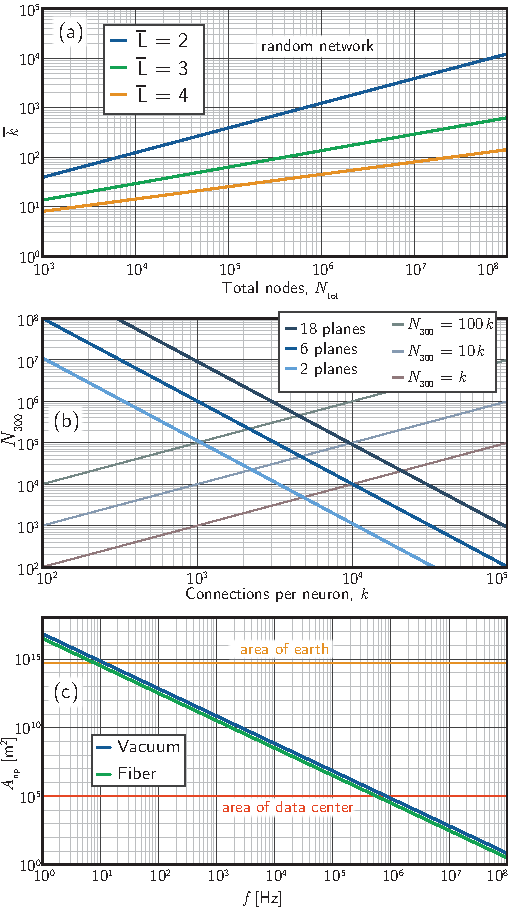
\includegraphics[width=8.6cm]{data_plots.pdf}}
	\captionof{figure}{\label{fig:data}Scaling considerations for optoelectronic neural systems. (a) The average number of connections per node required to maintain a give average path length across a random network as a function of the total number of nodes in the system. (b) The total number of nodes that can fit on a 300\,mm wafer as a function of the number of connections per node in the wire-limited regime \cite{ke1982}. (c) The area of the neuronal pool as a function of the frequency of neuronal oscillations assuming light-speed communication \cite{shICRC2018}.}
\end{figure}

\subsubsection{Clustering}
This analysis of average path length is relevant for quantifying a network's potential for information integration, but as we stated above, a neural system also depends on the ability for differentiated processing. Let us consider differentiation across various scales of the network. Ideally, no two neurons would behave identically, because this would not provide new information. Each neuron will fire preferentially in response to stimulus according to a tuning curve \cite{daab2001}. In practice, some redundancy is advantageous if a network is to rapidly gain confidence regarding the nature of a stimulus. Neural systems employ populations of neurons to represent certain pieces of information. The net activity across the population represents the presence or absence of a stimulus, and the variation in activity across the population represents uncertainty about the interpretation of the stimulus. In order for a certain population of neurons to predominantly exchange information locally and rapidly establish a consensus interpretation of a stimulus, the neurons in that population should comprise a preponderance of connections within the population. Groups of neurons with an abundance of connections within the group relative to connections external to the group form a community, and a clustering coefficient \cite{eskn2014,fa2007} is the simplest network metric. If node $a$ is connected to node $b$ and to node $c$, the clustering coefficient quantifies the fraction of cases in which node $b$ is also connected to node $c$. This metric provides insight into the tendency of neurons to form specialized communities with information processing differentiated from other parts of the network, and is first step toward analyzing the modularity of the system. 

\subsubsection{Small-world networks}
A random network has a low clustering coefficient, as the presence or absence of a connection between nodes $b$ and $c$ is, by definition, completely independent of the presence or absence of any connections to or from node $a$. Yet the networks of the brain\textemdash from the scale of neurons to the scale of connections between regions\textemdash show a high degree of clustering relative to a random network. As we have emphasized, neural information processing relies on both differentiated processing by local clusters and efficient integration of information across the network. We therefore expect neural systems to simultaneously achieve a high clustering coefficient and short average path length. A small-world networks is one with both of these traits \cite{wast1998}. We can introduce the small-world index (SWI) \cite{hugu2008} given by  $\mathrm{SWI} = \frac{\bar{C}/\bar{L}}{\bar{C}_{\mathrm{r}}/\bar{L}_{\mathrm{r}}}$, where $\bar{C}$ is the average clustering coefficient, $\bar{L}$ is the average shortest path, and the subscript, $\mathrm{r}$, refers to a random graph. Whether analyzed at the scale of populations of a few thousand neurons or at the scale of large regions of the brain, the networks demonstrate large $\mathrm{SWI}$, indicating that different populations of neurons represent different information, the activities of these populations can be efficiently communicated across the network, and  giving hints that brain architecture is hierarchical and modular.

\subsubsection{Modularity and hierarchy}
Anatomically, clusters in the brain were thoroughly described by Mountcastle in 1978 \cite{mo1978} before the concept of a small-world network had been introduced \cite{wast1998}. Mountcastle referred to the communities of neurons as mini-columns and columns. Imaging of biological neural systems with various techniques across all relevant length scales indicates modularity persists across multiple levels of hierarchy \cite{beba2017}. The clustering coefficient discussed above can be generalized to the modularity, $Q$, quantifying the degree to which the connections of a network depart from what would be expected of a random network to form partitioned communities \cite{rusp2010,beba2017}. For example, clusters of neurons are partitioned into mini-columns. At the next level of hierarchy, clusters of mini-columns are partitioned into columns. Clusters of columns are partitioned into brain regions. At the highest level of hierarchy in the brain, regions exchange information throughout the cerebral cortex and the thalamocortical complex that controls and coordinates operation of the largest modules comprising the brain. Neurons predominantly contribute to activity within their module, but they also must be able exchange information across partitions and up the information-processing hierarchy. Again we find differentiated, local processing combined with information integration across the hierarchical structure of the network. This neural information processing is enabled by a small-world architecture.

\subsubsection{Rentian analysis}
%\begin{figure} 
%    \centering{\includegraphics[width=8.6cm]{rentian_analysis.pdf}}
%	\captionof{figure}{\label{fig:rentian_analysis}Caption.}
%\end{figure}
We can quantify the ability of information to be communicated up the hierarchy by analyzing the number of connections penetrating various partitions of the network, referred to as Rentian analysis. Rent's rule states that the number of edges crossing the boundary of a partition ($k$) is related to the number of nodes within the partition ($n$) by a power law of the form
\begin{equation}
\label{eq:Rent}
k(n) = k_0 n^p,
\end{equation}
where $k_0$ is the number of edges emanating from each node (zeroth level of hierarchy), and $p$ is referred to as the Rent exponent. Rent's rule (Eq.\,\ref{eq:Rent}) was first observed in the context of VLSI circuits, and has also been shown to hold for biological neural circuits ranging from \textit{C. elegans} to the human brain \cite{bagr2010}. 

Depending on the system under study, the Rent exponent may vary, but is generally around 0.75 \cite{bagr2010}. We will demonstrate the use of Eq.\,\ref{eq:Rent} in Sec.\,\ref{sec:scaling}. The significance of the Rent exponent can be seen in its relation to the topological dimension, $D$. In Euclidean geometry, the surface area of a structure embedded in $d$-dimensional space is given by a power law of the form $s\sim v^p$. In general, the surface area $s$ scales as a length to the power of $d-1$, while the volume scales as a length to the power of $d$. Thus, in Euclidean geometry, $p = 1-1/d$, or $d = (1-p)^{-1}$. The same expression holds in fractal geometry \cite{ma1983,sc1991}, and in the case of Rentian scaling the topological dimension is related to the Rent exponent by $D = (1-p)^{-1}$, with $0 \le p \le 1$, so that $1 \le D \le \infty$. For $p > 2/3$, the topological dimension is larger than the embedding dimension, indicating that through a judicious implementation of input and output ports, information can flow through a network as if its components were connected in a higher-dimensional space. In the case of the brain, we find $D \approx 4$.

In any real network, it will only be possible to adhere to Eq.\,\ref{eq:Rent} across a certain domain of $n$. In the brain, consideration can apply from a single neuron up to the brain as a whole. Yet across this domain, Eq.\,\ref{eq:Rent} applies only piecewise, with discontinuities at certain partitions \cite{oz2004}. For example, we may expect Eq.\,\ref{eq:Rent} to hold from the scale of a single neuron up to the scale of a cortical column, but the connectivity patterns between columns are quite different than within, so we may expect a discontinuity at the scale of cortical columns, followed by a new expression of Eq.\,\ref{eq:Rent} with a different value of $p$, and perhaps a new interpretation of $n$ as the number of columns within a partition. Similarly in the domain of microelectronics, a multicore processor on a chip may obey Eq.\,\ref{eq:Rent} within each processor, with a discontinuity at the scale of the connections between processors. The wiring organization of VLSI circuits and the brain is statistically fractal, but not infinitely so. The limitations are purely physical.  

How does Rentian analysis inform our design of neural hardware? As we have emphasized, neural information is processed across a modular hierarchy. Rentian analysis quantifies the ability of information to be transmitted across partitions in the hierarchy. We conjecture that the ability for a neural system transmit more information across more levels of hierarchy will improve general intelligence. Therefore, between the neurons within a module, we expect that neural hardware should achieve high values of $D$ over a large range of $n$ before a discontinuity is necessary, so that multiple levels of hierarchy can be traversed efficiently within a module. Further, upon encountering a discontinuity, hardware must have a means of establishing another domain of Rentian scaling to efficiently collect and distribute information across more orders of hierarchy. Finally, we conjecture that the most intelligent neural hardware will provide this fractal scaling across as many levels of hierarchy as possible until the system finally reaches the limits set by the speed of communication. In Sec.\,\ref{sec:scaling} we will discuss these large-scale limits in biological and optical systems.

\subsubsection{Summary of spatial considerations}
The spatial structure of a neural system must comprise nodes with many edges to enable short path length across large networks. These nodes must also have high clustering to enable differentiated processing within modules. The information from these modules must be integrated across the hierarchy of the network, and the ability to do so is quantified by the topological dimension. Neural systems efficiently process information through the fractal use of space. Let us now consider their operation in time.

\subsection{Temporal dynamics of neural systems}
A neuron is a dynamical entity. It receives input from many afferent synapses, and it integrates this input over time. In a biological neuron, activity on a synapse results in a post-synaptic current into the receiving neuron. This current reduces the magnitude of the voltage across the neuron's cell membrane, and when that voltage is reduced below a threshold, the neuron produces an action potential, often referred to as a spike or pulse. This dynamical process of signal accumulation followed by bursting activity qualifies a neuron to be considered a relaxation oscillator. Before describing the temporal dynamics of neural systems in more detail, let us consider for a moment why relaxation oscillators are particularly well suited for cognition.

\subsubsection{Relaxation oscillators}
As we have mentioned, a defining aspect of cognitive systems is the ability to differentiate locally to create many sub-processors, but also to integrate the information from many small regions into a cohesive system, and to repeat this architecture across scales. A network of many dynamical nodes, each with the capability of operating at many frequencies, gives rise to a vast state space. As computational primitives that can enable such a dynamical system, oscillators are ideal candidates. In particular, relaxation oscillators \cite{st2015,mist1990,soko1993,lued1997,huya2000,bu2006,gile2011,vepe1968,cacl1981} with temporal dynamics on multiple time scales \cite{soko1993} have many attractive properties for neural computing, which is likely why the brain is constructed of such devices \cite{ll1988}. We define a relaxation oscillator as an element, circuit, or system that produces rapid surges of a physical quantity or signal as the result of a cycle of accumulation and discharge. Relaxation oscillators are energy efficient in that they generally experience a long quiescent period followed by a short burst of activity. Timing between these short pulses can be precisely defined and detected \cite{bu2006}. Relaxation oscillators can operate at many frequencies \cite{huya2000} and engage with myriad dynamical interactions \cite{lued1997}. The oscillator's response is tunable \cite{huya2000}, they are resilient to noise because their signals are effectively digital \cite{stgo2005}, and they can encode information in their mean oscillation frequency as well as in higher-order timing correlations \cite{pasc1999,thde2001,sase2001,stse2007,brcl2010,haah2015}.

\subsubsection{Binary communication}
For these reasons, we expect that any cognitive computing platform will be based on spiking neurons that behave as relaxation oscillators. Let us now consider some of the complex device functions that make neurons more capable of information processing than simpler relaxation oscillators. As mentioned above, communication between neurons is effectively binary\textemdash all or nothing. When a neuron produces an action potential, it propagates down the axon and branches throughout the axonal arbor. The signal propagates as a section of depolarization between the interior of the axon and the surrounding extracellular fluid. This depolarization opens pores in the membrane of the axon, allowing the flow of ions from the extracellular fluid into the axon, thus providing the electrical signal that will reach the synapses. Each time the action potential is generated, the behavior is nearly identical: the speed of propagation of the signal is set by the physical properties of the axon, the number of pores that open is very large and not noisy, and the signal that reaches the synapses is very similar from pulse to pulse. To further contribute to the digital nature of neuronal communication, the role of the action potential propagating down the axon is not to provide current to the post-synaptic neuron, but rather to begin a chemical cascade within the synapse that controls the signal amplitude. When the action potential reaches the synapse (pre-synaptic cleft), the action potential triggers the release of neurotransmitters into the synaptic cleft. These neurotransmitters diffuse through the fluid of the cleft, and bind to receptors on the post-synaptic cleft. These receptors then trigger the flow of current through the dendrite on which the synapse resides. This post-synaptic current carries the information that will be processed, first by the dendrite, then the dendritic arbor, and finally the soma. The action potential arriving at the synapse initiates the synaptic cascade in a binary, all-or-nothing manner, but the amount of current flowing into the post-synaptic dendrite depends on the state of the synapse, and it can take a continuum of values. Thus, communication in neural systems is digital (binary), yet information processing is analog. The synapse performs a digital-to-analog conversion, and the state of the synapse (which depends on many factors) determines the analog value entering into the computation performed by the dendrites and soma. 

\subsubsection{Short-term synaptic plasticity}
%\begin{figure} 
%    \centering{\includegraphics[width=8.6cm]{short-term_plasticity.pdf}}
%	\captionof{figure}{\label{fig:short-term_plasticity}Caption.}
%\end{figure}
The state of a synapse is affected by its activity over short and long time scales as well as external network factors. Neurons often signal in bursts (closely spaced sequences of spikes) \cite{iz2007}, and within a burst, the time between spikes is referred to as the inter-spike interval. Changes of synaptic response over time scales on the order of the inter-spike interval are referred to as short-term synaptic plasticity \cite{abre2004}. One key effect of short-term plasticity is to perform a temporal filter on an afferent spike train. This can be a high-pass, low-pass, or band-pass filter, as shown in Fig.\,\ref{fig:short-term_plasticity}. High-pass filtering results in only the first few pulses of a train being transmitted from the pre-synaptic axon to the post-synaptic dendrite. A synapse performing high-pass filtering reports to the post-synaptic neuron that the pre-synaptic neuron has begun to fire. Conversely, low-pass filtering results in synaptic response after the first several pulses of a train have occurred. A synapse performing low-pass filtering will not be active unless the pre-synaptic neuron produces a pulse train of a certain minimum duration, and therefore this synapse reports to the post-synaptic neuron when the pre-synaptic neuron has sustained bursting activity beyond a certain duration. Band-pass filtering combines these responses. A synapse performing band-pass filtering will only produce a response after an afferent pulse train exceeds a certain duration, and it will fall silent again after if the afferent pulse train continues beyond a certain duration.

These short-term filtering mechanisms enable synapses to report much more information to the neuron than simply the time-averaged rate of afferent activity. A neuron combining the signals from many synapses with various short-term responses has access to information regarding not just the average spike rates of the neurons from which it receives synaptic connections, but also regarding the initialization of bursting and the duration of spike trains.

\subsubsection{Long-term synaptic plasticity}
%\begin{figure} 
%    \centering{\includegraphics[width=8.6cm]{stdp.pdf}}
%	\captionof{figure}{\label{fig:stdp}Caption.}
%\end{figure}
Over time periods much longer than the inter-spike interval, the response of synapses can also change based on the activity of the two neurons involved in the synapse. A synapse that is more active will strengthen (long-term potentiation), and a synapse that is used less will weaken (long-term depression). This was the essential insight of Hebb in 1949 \cite{he1949}, a concept that developed in the subsequent decades \cite{bipo1998,somi2000} to account for the fact that long-term potentiation only occurs if the pre-synaptic neuron fires just before the post-synaptic neuron, indicating the potential for causality, while long-term depression is induced when the pre-synaptic neuron fires just after the post-synaptic neuron. This spike-timing-dependent plasticity (STDP) \cite{mage2012} plays a central role in memory formation and network adaptation. 

The physical mechanism responsible for STDP involves the growth and decay of neurotransmitter sources and receptors present at the synapse. These synaptic molecular machines (N-methyl-D-aspartate receptors, NMDARs) develop in response to the action potential arriving at the pre-synaptic terminal as well as the back-propagating signal from the post-synaptic neuron. The complex chemistry present at each synapse leads to a remarkable degree of diversity and adaptability in synaptic response.

By strengthening cooperative synapses, STDP adapts the structural network of neurons and their connections into functional networks embodying certain memories or computations learned over time based on the correlations of neuronal firing events. It has been shown that random networks with synaptic weights adjusted over time by STDP adapt into small-world networks \cite{shki2006}, maintaining efficient communication, and adding functional clusters specialized for specific computations. This is one example of the structural network of a neural system can be used to manifest multiple functional networks.

The functional clusters established via STDP have spectral signatures. A given functional cluster of neurons will have a specific pattern of activity, that may repeat in time. The period of this repetition will depend on the specific parameters of the circuit, and a large structural network comprising many highly connected neurons will have the potential to establish a vast repertoire of functional clusters with oscillations at many frequencies. Through STDP, the network can increase the activity of certain oscillations corresponding to highly utilized functional modules. If a certain stimulus has a probability of activating a certain functional cluster, the overtime, the action of STDP will enable the network to correlate that stimulus with the dynamical response of the cluster, and the stimulus will evoke the activity of the cluster with higher probability. In the language of dynamical systems, a specific cyclical response of the functional cluster is referred to as a basin of attraction \cite{iz2007,st2015}, and STDP ensures that relevant stimuli lead the network to the appropriate basin of attraction. This is function of an autoassociator, and it is an important form of long-term memory (\cite{bu2006} pg. 329).

Spike-timing-dependent plasticity makes use of correlations between firing activity of neurons to adapt the network into functional clusters \cite{shki2006}, store memories in dynamical sequences \cite{haah2015}, and strengthen circuits that demonstrate temporal patterns storing sequential memories (\cite{bu2006} pg. 318). But theoretical analysis finds that if STDP is the only long-term synaptic plasticity mechanism, memories are forgotten very quickly \cite{fuab2007}. Experimental analysis finds that synapses have multiple additional means to change how synapses adapt over time and activity to help retain memories \cite{ab2008}. These plasticity mechanisms are referred to collectively as metaplasticity.

\subsubsection{Metaplasticity}
While STDP adapts the strength of synapses (synaptic efficacy), metaplasticity adapts the rate at which synaptic efficacy changes over time and activity. For example, if a pre-synaptic neuron fires just before a post-synaptic neuron, the synapse connecting the two will be a candidate to experience long-term potentiation. But the \textit{probability} that the synapse actually does potentiate can be controlled by chemical signals within the synapse. Additionally, the \textit{amount} by which the synaptic efficacy changes is also subject to chemical modulation. 

The function of metaplasticity is to control which neural circuits adapt at a given time \cite{ab2008}. The receptors mentioned above (NMDARs) can be controlled based on a variety of factors related to network activity so that adaptability may be turned on and off in certain regions at certain times. This functionality is required of plastic synapses to keep them from too quickly losing the trace of a memory that is still needed. Experiments with humans indicate that forgetting occurs as a power-law function of time, \cite{wieb1991,wieb1997}, yet Fusi and Abbott have shown that memories are lost more rapidly than this if plastic synapses are presented with continual stimulus \cite{fuab2007}. They have proposed a model that achieves the observed power-law forgetting by introducing internal complexity to the synapses \cite{fudr2005}. In this model, each synapse has various states of efficacy (weak and strong synaptic weight), but it also has additional internal states with the same efficacy. The difference between these states is the probability with which the efficacy will change due to future plasticity events. 

Metaplasticity provides a network with the means to to enable some regions to adapt at a given time, under a given stimulus, while other regions are unchanged at that time, under that stimulus. Further, metaplasticity provides a means by which some synapses within a region may change very rapidly to adapt to a new stimulus, while other synapses in the same region may change slowly or not at all when presented with the same stimulus. We expect that an intelligent neural system have the capability to immediately learn in response to new information, but also to maintain a lasting representation of all that has been learned through the network's existence even in the presence of continually varying input. Metaplasticity is an important means by which rapid learning in conjunction with long memory retention can be achieved. As stated by Abraham, ``...these metaplasticity processes represent a major form of adaptation that helps to keep synaptic efficacy within a dynamic range and larger neural networks in the appropriate state for learning.''

\subsubsection{Homeostatic plasticity}
To conclude this discussion of synaptic plasticity mechanisms, we note that short-term plasticity adapts based only on the activity of the pre-synaptic neuron, while STDP adapts based on correlations in the activity between pre- and post-synaptic neurons. The mechanism of homeostatic plasticity \cite{cube2012} adapts synaptic weights based only on the activity of the post-synaptic neuron. Homeostatic plasticity (also referred to as the Bienenstock-Cooper-Munro (BCM) model) adjusts the synaptic weights of synapses incident upon a given neuron based on a sliding temporal average of the recent firing activity of that neuron. Such a mechanism provides a means by which neuron and network activity can be maintained within useful limits and dynamic range can be maximized.

\subsubsection{Dendritic processing}
We have discussed how STDP leads to the formation of functional clusters within a network based on the history of correlated neuronal activity. But what if the network wishes to isolate specific functional clusters on time scales as short as an inter-spike interval? Or what if we wish to endow a neuron with the ability to respond not only to activity in single synapses, but rather to integrated activity from specific clusters of synapses, or to specific sequences of activity within a cluster of synapses? Dendritic processing enables these functions.

Dendritic processing refers to the intermediate, nonlinear transfer function performed by dendrites between individual synapses and the neuron as a whole \cite{stsp2015}. The dendritic arbor is a complex, branching structure on which most of a neurons input synapses make their connections. The dendritic branches that comprise the arbor have passive and active properties that allow them to perform various computations. The dendritic arbor can thus be modeled as a network of multiple independent threshold units that integrate signals and produce dendritic spikes upon reaching threshold \citep{sava2017}.

For example, consider a dendrite with two synapses. If the post-synaptic current into the dendrite is sufficient to produce a dendritic spike, and if this dendritic spike has the same form whether one or both synapses fire, the dendrite performs the OR operation. If both synapses are required to fire to produce a dendritic spike, it performs the AND operation. The current generated in a dendritic spike propagates only a short distance along the dendritic tree, into the next dendritic compartment closer to the cell body, and the current decays with an exponential time constant. Thus, dendrites can perform basic logical operations with a temporal component, and activity closer to the base of the dendritic tree at the cell body integrates information from a larger number of inputs. 

In addition to the simple two-synapse Boolean operations described above, it has been proposed that 

Dendritic processing may even play a central role in learning as well. It appears to be the case that modification of NMDA receptors involved in STDP is governed by the production of dendritic spikes, and it is not required that the neuron fire in order for synaptic potentiation or depression to occur. These dendritic processing functions, including integration and thresholding, basic logical operations, sequence detection, and role in learning, indicate several means by which the devices comprising neurons and neural systems perform complex operations to maximize the ability of each neuron to utilize the information it is presented. In light of all this complexity, how should we mathematically model these devices?

\subsubsection{Which model of neuronal dynamics to use?}

\subsubsection{From devices to populations}

\subsubsection{Neuronal avalanches}

\subsubsection{Entrained oscillations and synchrony}

\subsubsection{Cross-frequency coupling}

\subsubsection{Fractal use of space and time}


\begin{itemize}
\item get into a tad of history here, analogous to Turing/von Neumann
\end{itemize}

General intelligence: The ability to place a wide variety of information into a coherent context so that the behavior of the relevant parties can be understood and predicted.

\subsection{Summary of neural information}
Von Neumann suspected the existence of a more subtle and powerful language of information employed by the human brain. Neuroscience has elucidated many of the principles of this language. Let us attempt here to summarize the salient elements that should guide neural hardware design. Given the complexity of the subject and the rapidly evolving state of neuroscience, we expect time to bring corrections to these concepts, yet the foundations of these concepts do seem well established.

The model from neuroscience informing the hardware presented here is as follows. Each neuron attempts to gain access to as much information as is physically possible about the activities of the other neurons in the network. Each neuron gains access to pieces of this information based on the temporal filter it performs. For example, a given synapse (or pair) can pas on information about the rate, rising edges, falling edges, temporal correlations, or sequences output from any neuron (or pair) in the network. In the temporal domain, we assume the signals can each be given a distinct exponential decay constant. Each synapse then has the information to answer a question, such as, how much has neuron $i$ been firing in the last $\tau_{ij}$ seconds? Or, how much has neuron $i$ been bursting, and then quiescing, and then bursting again in the last $\tau_{ij}$ seconds? 

The answers to these questions must pass through the dendritic arbor. Each dendrite contains information received from one or a number of synapses coupled to the dendrite. The net information contained in the dendrite may be able to answer a question such as, how much have neurons $a$, $b$, and $c$ collectively been firing in the last $\tau$ seconds? Or, how many of a particular subset of 10 neurons in cluster $q$ have stopped firing in the last $\tau$ seconds? 

When under the influence of inhibitory neurons, a dendritic compartment will be quiet. Upon the release of inhibition, the dendritic compartment reports to the neuron the answer to the question it knows how to answer by transmitting an analog signal in the form of current that modifies the neuron's membrane potential. Each segment of the dendritic arbor performs a nonlinear transfer function on the signals from the synapses connected to that segment, and the neuron itself performs a nonlinear transfer function on the signals it receives from across its dendritic arbor. The neuron's nonlinear transfer function is to produce a pulse (an action potential) when the membrane potential of the soma reaches a certain threshold value. This pulse is communicated through the neuron's axonal arbor to all the neuron's downstream connections as a digital signal, wherein the presence of the pulse informs all downstream connections that under the present network conditions, the activities on all that neuron's dendrites were sufficient to induce firing, and the amplitude of the pulse is not used to encode information.

In this picture, the excitatory (pyramidal) neurons are a knowledge base that can be queried by the inhibitory interneuron network. The net objective of the network is to be able to identify as many correlations as is physically possible across space and time. In space, these correlations are limited by network path lengths. In time, correlations are detectable over time constants of synapses and dendrites. To identify correlations over longer times than this (such as the lifetime of the entity), the logic of synaptic plasticity and metaplasticity come into play \cite{fudr2005,fuab2007}. Note that this model of inhibitory query of pyramidal neurons is readily scalable across arbitrary partitions of the network, so the basic informational principles are continuous from the scale of local networks up to the system as a whole. This is uniquely enabled by the fractal use of space and time.

We conjecture that the probability of observing a neuronal avalanche accessing the information in $s$ dendritic compartments scales as $P(s)\sim s^{-\alpha}$. During oscillatory behavior, inhibitory neurons sample specific dendrites in an intentional, controlled manner at a frequency $f_{\theta}$, so that the information contained in the collection of all synapses, dendrites, and neurons active in the functional network resonant at $f_{\theta}$ can be integrated across partitions of the network to be incorporated in computations a higher levels of network hierarchy. The mechanisms for this coherent information access and integration include cross-frequency coupling, wherein local activity occurring at higher frequencies $f_{\gamma}$ is modulated by slower frequencies $f_{\theta}$, with the phase of the higher frequency activity being well-defined relative to the phase of slower frequencies. Such network-wide information integration through multi-scale activity across space and time is thought to be necessary for cognition \cite{bu2006}, perhaps by enabling access to the global neuronal workspace \cite{ba1988,de2014}.

To summarize the summary, a single neuron extracts as much information as it can from its neighbors, and it transmits as much as it can to its neighbors through its activity in various effective network contexts established by the state of the dendritic arbor as configured by the inhibitory interneurons. A cluster in the network attempts to answer as many questions as it can about its inputs, and it attempts to communicate this information across the network to as effectively as possible, and so on up the hierarchy of network partitions. A network of inhibitory neurons samples the information from synapses and dendrites in myriad combinations, in principle answering any question that could be reasonably posed regarding a stimulus that could be physically presented to the entity. 

This model of neural information processing bears a resemblance to a Turing machine. Turing's goal was to make a machine that could answer any question that could be asked within the axioms of its system (universal while not violating G\"{o}del), and the goal here is essentially the same. Yet in addition to the Turing machine behavior, wherein the network acts as an oracle, an intelligent neural system should also be able to ask its own questions by formulating an output that generates a response from an intelligent or inanimate agent so as to gain new information. In addition to generating an entity that is universal in the sense defined by Turing, we aspire to create machines that are intelligent in the sense that they can engage in self-directed learning. Such a machine will be able to answer our questions, but also have a mind of its own.

\section{\label{sec:electronics}Semiconductor electronic neural systems}

\begin{itemize}
\item Mead
\item shared communication infrastructure
\item address-event representation (Bigelow: ``by means of explicit systems of tags characterizing the basically irrelevant geometric properties of the apparatus, known as `addresses'. Accomplishment of the desired time-sequential process on a given computing apparatus turns out to be largely a matter of specifying sequences of addresses of items which are to interact.'' \cite{bi1955})
\item connectivity/speed tradeoff
\item synaptic, dendritic, and neuronal functionalities: emulating neural behavior with digital systems.
\item connect back to von Neumann: stepping through a differential equation in time with a Turing machine rather than leveraging devices that physically manifest the differential equations of interest
\item hardware for universal computing with a Turing machine is not efficient for neural information
\item memristors: really crappy synapses
\item application spaces: deep learning, mobile devices, IoT; neuro-inspired, but not really neural computing
\item mention Mead, sub-threshold transistor IandF isomorphism
\item The distributed von Neumann approach still effectively steps through differential equations numerically. We advocate for hardware that actually lives through the response modeled by the diff eqs. 
\item in many CMOS manifestations, each processor core follows the instructions in discrete time that cause it to behave as if it obeyed certain neural differential equations, but the underlying devices do not actually obey those equations. They simply obey the differential equations describing carrier dynamics in semiconductors. Mead attempted to utilize these semiconductor dynamics in analog to behave as neurons, but this has not met with much success, and contemporary approaches more often utilize a digital model of the analog neural system.
\item mixed-signal approaches
\item contention delay is incompatible with neural information processing
\item CMOS neuro: one aspect of problem is inefficiency of using Turing machine to behave as a neural system
\end{itemize}

\section{\label{sec:superconductors}Superconductor electronic neural systems}

\begin{itemize}
\item JJ basics
\item superconducting digital (going right for the von Neumann architecture, binary, solution to diff eqs)
\begin{itemize}
\item IBM latching logic
\item Likharev
\item victorious march of CMOS
\item third wave: IARPA/C3
\end{itemize}
\item JJ neurons (Japan, Segal, Schneider, that recent theory paper)
\item still, communication problems, fan-out
\end{itemize}

\section{\label{sec:optoelectronicNeurons}Optoelectronic synapses, dendrites, and neurons}

\begin{itemize}

\item light easy to use for long haul, but chip scale?
\item occurs in the context of silicon photonics evolution, soref and bennett, Luxtera, vladimir

\item general concept: communication between neurons is photonic; when a neuron spikes it must either generate or modulate light; throughout, speed, size, power all co-optimized

\item first key choice: generate or modulate

\item modulate:
\begin{itemize}
\item requires cw light running at all times ($x_{dB/cm} = 1; y_{dB/s} = 100*x_{dB/cm}*c; q_{dB} = 3; t_s = q_{dB}/y_{dB/s}$, for 1\,dB/cm propagation loss, 3\,dB of the light is lost every 100\,ps)
\item requires frequency tuning, most likely
\item cross talk of neurons on the same bus
\end{itemize}

\item generate:
\begin{itemize}
\item requires light source at every neuron
\item requires unprecedented optoelectronic integration, million sources and a billion detectors on a wafer
\item must be very low capacitance
\item seems like only a silicon light source will suffice, but this would require cryogenic operation
\end{itemize}

\item second key choice: establish synaptic weight in the photonic or electronic domain?

\item photonic domain:
\begin{itemize}
\item This choice has several important ramifications for hardware and information processing. Regarding information processing, it is usually assumed that neural communication is digital: the presence or absence of an action potential is a binary one or zero, and the amplitude of the action potential is not encoding information. When adjusting the synaptic weight in the photonic domain, this is not the case. The number of photons reaching a neuron through a synaptic connection becomes an analog variable, and it is subject to shot noise, in addition to any noise mechanisms present in the detector. The signal-to-noise ratio of shot noise improves with $\sqrt(N_{\mathrm{ph}})$, where in this case $N_{\mathrm{ph}}$ is the average number of photons, so establishing weights in the photonic domain introduces an energy/noise tradeoff. Setting weights in the photonic domain also has the disadvantage that photons are discarded by attenuation at weak synaptic weights. Thus, by setting synaptic weights in the photonic domain, we place a burden on light sources to produce large numbers of photons to minimize shot noise, and we discard photons when they are attenuated at weak synapses. In this mode of operation, light is used for communication, but it is also used for the important computational operation of applying the synaptic weight.
\item these objections notwithstanding, to our knowledge, all except one optoelectronic neural approach proposed to date sets weight in photonic domain
\item specific instances: mzi (no STDP, poor spatial scaling, cross-talk); wdm (limited number of channels, cross-talk with rings on master ring, demands on sources); mzi and wdm (thermal tuning hopeless for scaling, no plasticity mechanisms proposed); phase change synapses (at least don't dissipate steady state, still power lost due to variable attentuation, small footprint, Hebbian learning possible, but STDP not likely, meta, short term also doesn't look promising)
\end{itemize}

\item electronic domain:
\begin{itemize}
\item By contrast, if we establish synaptic weights in the electronic domain, light is used exclusively for communication, and communication remains entirely digital. The presence of an optical signal can be used to represent an all-or-none communication event. In this case, the detector and associated electronics must be able to achieve a variable synaptic response to identical photonic pulses based on the configuration of the electronic aspects of the circuits. In this case, we expect that a neuron will send, on average, $N_{\mathrm{ph}}$ photons to each of its downstream synaptic connections. Due to shot noise, each downstream connection will receive $N_{\mathrm{ph}}\pm\sqrt{N_{\mathrm{ph}}}$ photons, and the detector circuit must be configured to implement a synaptic response if a threshold of $N_{\mathrm{th}}$ photons is detected. After detection, the electronic response must vary depending on the synaptic weight, independently of the precise number of photons that was detected. It is in this electronic response that the signal becomes analog again. Whereas setting the synaptic weights in the photonic domain places a larger burden on light sources, setting the synaptic weights in the electronic domain places a larger burden on detector circuits. One must achieve a detector circuit that converts light pulses to electrical current or voltage, and the amount of electrical signal must be largely independent of the number of photons in the pulse, depending instead on reconfigurable electrical properties of the circuit, such as bias currents or voltages. These reconfigurable bias currents or voltages then represent the synaptic weights, and the task of a neuron's light source is simply to provide a roughly constant number of photons to each of its downstream synaptic connections. For energy efficiency, the number of photons necessary to evoke a synaptic response from the detector ($N_{\mathrm{th}}$) should be made as low as possible to make the job of the light source as easy as possible. $N_{\mathrm{th}}$ cannot be made lower than one, as the electromagnetic field is quantized into integer numbers of photons.
\item only know of one system where electronic domain has been proposed: soens
\item basic functionality
\item stdp
\item meta
\item homeo
\item short-term
\end{itemize}

\item neuronal computation: reaching threshold
\begin{itemize}
\item differentiate between state-based and spiking
\item main considerations here are energy/power
\item how much energy is required to generate a pulse or drive a modulator? 
\item how much light must be made/moved to drive all downstream synaptic connections? 
\item how fast can pulses be generated (refractory period)? 
\item how long can neurons remember (leak rate)? 
\item what is range of spike rates? what is expected power?
\end{itemize}

\item somewhere in here, comparison of detectors (going cold costs 500x for carnot, but gains 2000x for detector sensitivity)
\item related, comparison of sources (going cold reduces how many photons must be made, but most importantly, if it means a silicon light source can work for this project, it is a game changer)

\item inhibition, gotta have a plan

\item dendritic processing
\begin{itemize}
\item intermediate nonlinearities
\item direction attention with inhibition
\item sequence detection
\item how can any of this happen in the photonic domain?
\end{itemize}

\item room temp vs cryo
\begin{itemize}
\item sources (cryo enables Si sources. for large-scale integration, process simplicity brings tremendous advantage)
\item detectors (A SiGe photodetectors needs about $10^4$ photons in 100\,ps to respond; efficiency of SNSPDs, low-noise of SNSPDs, simplicity of fabrication, and excellent operation in conjunction with JJs)

\end{itemize}

\end{itemize}

\section{\label{sec:scaling}Large-scale optoelectronic systems}

\begin{itemize}
\item unprecedented integration of photonics and electronics in a scalable process that can be implemented with existing infrastructure--change a few implant conditions, swap out a few sputtering targets, improve BEOL dielectrics for photonics
\item communication on various length scales, multi-planar on wafers, wafer-to-wafer vertical and lateral, fiber white matter
\item feasibility of brain scale
\item why si if no transistors?
\begin{itemize}
\item III-V substrates should be pursued as well. Our group is working on this, initial anecdata indicates similar efficiency
\item big problem is fab. wafers are harder to scale, material harder to purify, oxide not as good for waveguide cladding. Similar consideration to mosfet gate. Overall manufacturability
\item may eventually use transistors for perhaps faster refractory period
\end{itemize}
\item ultimate limits
\end{itemize}


For general networks, the algorithm by which partitions are identified can be made mathematically rigorous from a network theory perspective \cite{oz1992,oz2004}. For the analysis at hand, we consider the partitions of the network we have assigned in the hierarchy. For example ... (minicolumns, mesocolumns, macrocolumns on a wafer(s); multi-columnar modules, ...) 

\section{\label{sec:applications}Application spaces}

\begin{itemize}
\item original applications of computing
\begin{itemize}
\item cryptography
\item weather
\item bombs
\item numerical solution to arbitrary diff eqs
\item from Turing, AI
\item now, apply to nearly all aspects of modern life
\end{itemize}
\item here, following neuroscience applications 
\begin{itemize}
\item vision systems
\item language processing
\item motor control
\item may lead to Turing's vision of an AGI one can interact with
\end{itemize}
\item others, unique to large-scale neural systems and/or superconducting optoelectonic
\begin{itemize}
\item internet monitoring/simulation
\item society simulation
\item genetic analysis/evo devo
\item neuroscience and dynamical systems
\item quantum/neural hybrid systems (Bayesian discussion)
\end{itemize}
\end{itemize}

\section{\label{sec:outlook}Outlook}

\begin{itemize}

\item circle back to Turing and von Neumann, their interests in machine intelligence and modeling computation after the brain
\item circle back to digital vs neural, superconducting optoelectronics brings communication and spiking nonlinearities

\item why go to all the trouble?
\begin{itemize}
\item this technology will only be pursued if it can do something that nothing else can do
\item but it can, and what it can do is very important
\begin{itemize}
\item exceptional complexity for experiments in network information, neuroscience models
\item quantum/neural hybrid systems
\item scaling beyond what is possible with other methods, perhaps the smartest machines on the planet
\item computing has shaped economy and society since its inception
\item powerful scientific tool
\item foundational questions about thought and consciousness amongst the most intriguing and important in modern science
\end{itemize}

\end{itemize}

\end{itemize}

\vspace{3em}
We conjecture that Lovelace and Turing were both right. She was right that computing machines as they were known to her, and with the serial processing Turing proposed, really are not up to the challenge of thinking. And he was right that a machine can be capable of thought and learning like a child, but to do so, a modality of operation significantly different from the sequential instruction execution of the Turing machine must be employed.


\vspace{3em}
Working in the field of beyond-CMOS computing hardware, one quickly absorbs the mantra: never underestimate CMOS. Working the the field of hardware for AI, one quickly absorbs the wisdom: never underestimate the brain. We recognize the audacity in proposing hardware to outperform CMOS for any task. Yet we think the arguments presented here make the case that it is worth pursuing silicon-based technology with superconductors, light sources, and waveguides instead of transistors and electrical interconnects for cognitive neural systems. Does this mean we are confident such hardware will lead to beyond-human intelligence? Not at all. We understand CMOS, and we know what its limitations are likely to be. But the brain maintains important secrets, even after hundreds of years of inquiry. We have laid out an architecture that achieves fractal scaling over many orders of magnitude, and appears promising for enabling communication across the hierarchy at speed far greater than biological systems. And we have tried to respect the complexity of synaptic, dendritic, and neuronal functionalities in our circuit concepts. But it is possible that the subtleties of neuronal devices and architectures are more clever than we presently comprehend, and the structures we have discussed\textemdash from circuits to systems\textemdash will not achieve the nuanced information processing that leads to advanced cognition. For example, at the device level, synapses communicate with many neurotransmitters that can be modulated independently and affect information processing differently. At the architecture level, the thalamus coordinates information processing and enables access to the global neuronal workspace in a masterful manner that unifies the signals from many brain regions into a coherent cognitive moment. It is not clear that the circuits presented here will achieve comparable complexity, and it is not clear that we will soon understand how, with optoelectronic systems, to implement something like the thalamocortical complex that integrates information across the entire network architecture. It is our perspective that progress beyond the present state requires a significant experimental effort. Hardware must be devised, and networks must be observed. Only then will we find the limits of what can be made and how well it can process information.

\vspace{4em}
Misc. notes:

\vspace{4em}
\begin{itemize}
\item origins of modern computing intertwined with WWII
\item Turing: interests, universal computation, computability, Turing machine, serial, cryptography
\item von Neumann: interests, universal computation, numerical investigation of numerous physical problems, numerically solving differential equations, digital computing, memory storing data and instructions, von Neumann bottleneck
\item cryptography leads to creation of Turing machines one side of the Atlantic, numerical analysis of nuclear weapons leads to creation of Turing machines on the other (Dyson, pg 257)
\item Shannon: communication, information in data streams, again focus is on serial information processing
\item computing hardware: vacuum tubes, punched cards lead to silicon microelectronics, si uniquely suited to accomplishing digital computing, von Neumann architecture still going strong in si
\item communication hardware: ethernet for pretty big networks, fiber-optic cables replacing telegraphs under the atlantic
\item silicon photonics is where these two meet: light for commmunication, electronics for computation, maintaining the von Neumann architecture, WDM across the von Neumann bottleneck
\item Turing's discussion of ingenuity and intuition (Dyson pg. 252): digital all ingenuity, brute force search; neuro brings intuition back and honors its role; populations of neurons enable intuition to be based on Bayesian inference rather than random guesses.
\item Turing says ``ingenuity replaced by patience''. This is very much what happens in digital neuro. Brute search takes to long to enable neural information processing.
\item computing, communication theory, and cryptography all advanced significantly during and in response to WWII. The 80 years from 1938 to 2018 have seen the emergence of transformative technologies in these fields. Much contemporary work follows in these veins. For example, the goals of a universal quantum computer are very similar to Turing's universal calculator, with the addition of quantum physics to dramatically increase the speed of certain algorithms. Because quantum states are fragile and subject to decoherence, quantum systems strike us as very poorly suited to perform the serial operations of a Turing processor requiring writing and reading to reliable memory. Nevertheless, the requirement for cryptography in a world where trust is unfounded is sufficient motivation for many to pursue quantum computers, if for no other reason than to perform Schor's algorithm.
\item Grover's search algorithm is another motivator, again following Turing's line of reasoning to replace intuition with ingenuity, and ingenuity with brute search. The problem is the physics and hardware we have at our disposal make it very difficult to realize machines capable of performing these operations efficiently. 
\item In addition to limitations resulting from the fact that it is hard to implement quantum computers in hardware, some problems simply do not map well onto Turing machines, no matter the machine's complexity. Embracing the duality of ingenuity and intuition, as a neural system does, is increasingly useful for solving many of our present problems, including those of national security and defense, and extending into realms of medicine and science.
\item ``The paradox...to understand.'' \cite{dy2012} pg. 263.
\end{itemize}


\vspace{2em}
At different times, a neuron firing is known by other neurons to mean different things.

\vspace{3em}
Reasons to publish

1. New/early/infancy; significant development required, both concept and hardware
2. If soens ever did prove feasible, crossover would be Bostrom's slow category
3. Will require concerted effort, probably at least 100s of people, money, foundry
4. A specific hardware proposal has the potential to offer a useful case study, perhaps leading to preparedness
5. I am an employee of the Federal Government in service of the US taxpayers, and I have an obligation to publish my research.
6. If a superintelligence powerful enough to rapidly overcome us decides in fact to do so, it may have good reason to do so
7. I strongly doubt if a fast takeover transpires. That would
8. If such a technology is a threat, the sooner we are aware of it's potentiality the better

Reasons to expect soens to be slow (at least decades)

1. Need new hardware, at least 10 years
2. Need device and architecture improvements, theory and experimental capabilities, breakthroughs in understanding how to use such systems
3. Expensive, at least \$1B for human-brain scale
4. Progress will come in distinct hardware generations. We can ensure we don't produce the next iteration until we are ready
5. It will take a movement of historical proportions to realize beyond-human intelligence with soens, there is no risk of stumbling abruptly across the finish line

%In the neural system, recent computations are effectively stored at synapses

%Light is excellent for communication. Fiber optic links carry vast quantities of information across continents and between data centers. An important question in modern computing is: what is the shortest distance over which photonic communication will displace electronic interconnects? Optical links between racks in data centers are becoming common \cite{}. Major companies are investing seriously in photonics in the package. Monolithic optical links between processor and memory fabricated in a 45-nm CMOS node with no in-line changes have been demonstrated \cite{suwa2015}. A primary challenge affecting further chip-scale electronic-photonic integration is the continued difficulty of achieving a light source implemented on silicon that is robust, efficient, and economical.
%
%In parallel with the hardware considerations affecting optoelectronic integration are questions related to architecture. A prominent theme emerging since clock speed leveled off in 2003 \cite{} is parallelism. Computation is increasingly distributed among more processor cores. Many-core architectures continue to expand into on-chip networks, in some cases resulting in highly distributed, brain-inspired systems \cite{}. As compute grows more distributed, communication across interconnection networks becomes a bottleneck. The demand for energy efficient communication bandwidth has been a major driver of on-chip photonics.
%
%The major drivers for brain-inspired computers fall on a spectrum: energy and algorithmic efficiency for deployable applications reside on one side of the spectrum, and artificial general intelligence (AGI) resides on the other. Knowledge gained from neuroscience informs us that systems with general intelligence will benefit from very large numbers of computational elements as well as extreme communication between them. It is our perspective that hardware incorporating light for communication between electronic computational elements combined with an architecture of distributed optoelectronic spiking neurons will provide tremendous potential for AGI. Considerations pertinent to the realization of such a technology are the subject of this article.
%
%
%\section{\label{sec:sructureAndFunction}Structure and function across space and time}
%To guide the design of hardware for AGI, we must simultaneously consider operation across spatial and temporal scales. In Fig.\,\ref{fig:complexityAcrossScales}, we chart the structures present on various length scales and temporal scales for biological and optoelectronic hardware. The human brain has features spanning roughly eight orders of magnitude in size, from a nanometer to a tenth of a meter, with correlated dynamical activity across four orders of magnitude, from below 1\,Hz to around 600\,Hz. There are several types of optoelectronic neural systems, and we have proposed a specific approach we see as most conducive to large-scale implementation for AGI \cite{sh2018a}. These optoelectronic networks are likely to have features as small as 100\,nm and potentially extend up to many kilometers. Dynamical activity may be present from slow temporal scales up to 20\,MHz (30,000 times the maximum speed of the brain) for networks measured in kilometers. To enable such spatial and temporal scaling, fractal properties must be employed.
%
%Information processing in neural systems employs local clusters of neurons to represent specific features, and the information from these clusters must be shared with other regions of the network to form a multifaceted representation of a complex stimulus. Structurally, this information processing is facilitated by networks with a high clustering coefficient \cite{} yet also an average path length nearly as short as a random graph \cite{eskn2015}. Such graph structures are referred to as small-world networks \cite{wast1998}, and are ubiquitous throughout the brain \cite{sp2010}. To achieve small world networks, long-range connections are necessary. In a random network, near and distant connections are equally probable, so the average path length across the network is small, representing a lower limit on path length for a given number of edges connecting a given number of nodes. In Fig.\,\ref{fig:data}(a) we plot the number of edges required per node to achieve a given average path length as a function of the number of nodes in the network \cite{}. Consider the case of a network with one million nodes. We see from this plot that if we wish to maintain a path length of two, each node must make, on average, one thousand connections. For the case of a network with 100 million nodes, each node must make 10,000 connections. This is similar to the case of the hippocampus in the human brain, with nearly 100 million neurons, each with 10,000 or more synaptic connections. Maintaining a short average path length across the network is critical to enable efficient information integration, and this appears to be a major factor driving the extensive connectivity of biological neural systems. In the present context, this motivates us to conceive of artificial hardware capable of supporting comparable connectivity, which leads us to consider using light for communication.
%
%In addition to structural considerations pertinent to information integration across space, we must also consider how information propagates across time in neural systems. The computational primitives best equipped to integrate information across space and time are neurons, relaxation oscillators that encode information in the timing of their pulses. One of the most impressive aspects of neural information processing is that the same structural network can be used at different times in different contexts to form myriad functional networks. Over time scales on the order of neuronal inter-spike intervals, this is accomplished in two ways. First, short-term synaptic plasticity enables synapses to rapidly adapt in response to network activity, essentially resulting in temporal filtering of afferent spike trains \cite{abre2004}. Second, inhibitory neurons working in conjunction with dendrites can silence or give voice to specific synapses, clusters of synapses, or neurons depending on the local and global activity of the network. In addition, dendritic processing, wherein the dendritic arbor performs intermediate, nonlinear transformations between synapses and the soma, enables utilization of timing information \cite{vagu2005}, detection of sequences of activity \cite{haah2015}. Over time scales long compared to an average inter-spike interval, long-term potentiation and depression of synapses is employed to store memories \cite{} and adapt the network to a small-world architecture \cite{}. Learning in the presence of a continually changing environment while maintaining long-term memories is achieved through spike-timing-dependent plasticity (STDP) \cite{somi2000} and metaplasticity \cite{ab2008}. Neurons employing inhibition, dendritic processing, short-term, and long-term synaptic plasticity can make efficient use of a structural network by dynamically adapting on time scales from an inter-spike interval to the lifetime of the system. We refer to these synaptic, dendritic, and neuronal functions collectively as the computations performed by the neurons, and the standard threshold/spike operation is included. While light is excellent for communication with high fan-out between neurons in a cluster as well as across distant regions of a network, electrical circuits are better equipped to perform the computations necessary for adapting a vast structural network into dynamical functional networks useful for information processing. 
%
%In neural information processing, space and time are interrelated. This is evident both in oscillatory behavior such as cross-frequency coupling as well as anharmonic behavior such as neuronal avalanches. Cross-frequency coupling enables fast activity of local clusters to be modulated and sampled on slower time scales across larger regions of the network \cite{}. Cross-frequency coupling is enhanced during activities that require attention and coordinated response of multiple brain regions, and is one technique by which the brain utilizes oscillations at various frequencies for information integration \cite{bu2006}. Neuronal avalanches, on the other hand, are present as background activity even when attention is not directed to a particular subject, and can be anharmonic in nature \cite{}. Yet, similar to cross-frequency coupling, such cascades of spiking activity communicate across local, regional, and global partitions of the network. We denote by $s$ the number neurons involved in a neuronal avalanche. Neural activity across many species, brain regions, and contexts shows the probability of observing an avalanche of size $s$ follows a power law: $P(s)\sim s^{-\alpha}$. Systems with a power-law distribution of neuronal avalanches demonstrate self-organized criticality \cite{}, which maximizes the dynamic range of the system \cite{}. Such a power-law dependence has the important property that the ratio of number of events of size $qs$ to the number of events of size $s$ is simply $q^{-\alpha}$, independent of $s$. For this reason, such a distribution is referred to as ``scale-free'', and is self-similar, or fractal, across spatial and temporal scales. 
%
%Related to the fractal scaling of neuronal avalanches, neural systems are fractal in space in that they obey power-law scaling of connectivity \cite{bagr2010}, as well as in time in that they demonstrate power-law power-spectral density \cite{budr2004}. Fractal properties of neural systems are crucial to operation. Fractal systems can continue to scale, with dynamics constrained only by the physical hardware and spatial extent of the system rather than by the ability to communicate across the architecture \cite{plth2007}. Such scale-free systems can efficiently integrate information from local clusters to vast networks, while enabling correlations across wide regions of space and long periods of time. We conjecture that intelligent systems must achieve small-world structural networks with many nodes, and the computational elements comprising the nodes must support adaptive, dynamical responses on many time scales to fully utilize the structural networks for functional computation. We further conjecture that light is most capable of achieving communication across the structure of the network, while electronic circuits are most capable of achieving the dynamical activity necessary for computation. Based on these consideration, we expect a hardware platform capable of AGI to combine the strengths of photonic communication with electronic computation to integrate information in neuronal avalanches from small, local clusters on a silicon wafer to the light-cone-limited region of space across which light can travel in a network oscillation cycle.  
%
%\section{\label{sec:synapsesDendritesAndNeurons}Optoelectronic synapses, dendrites, and neurons}
%The device factors mentioned above are not quirks of the biological world, but rather are some of the reasons brain computation is so complex and efficient. Short-term plasticity produces information about spike train rising and falling edges and guards against runaway activity. STDP strengthens correlations between neurons that fire constructively and dampens connections that waste energy. These mechanisms have been shown to adapt random structural networks into complex functional networks with small-world architecture and neuronal avalanches indicating maximal dynamic range due to criticality. Dendritic processing in conjunction with inhibitory interneurons makes efficient use of the complex spatial network by dynamically activating a wide range of functional networks. To achieve these myriad computational functions, optical interactions are inadequate. The complexity of electronic circuits is required. 
%
%We envision optoelectronic hardware with photonic communication along waveguides playing the role of axons, and computation performed in electronic synapses, dendrites, and neurons. We make two more choices to specify the platform. Detectors must respond to single photons for maximal energy efficiency. Superconducting-nanowire single-photon detectors (SNSPDs) are the clear choice for this application, with very low dark counts, near-zero static power dissipation, and scalable integration \cite{shbu2017b}. An SNSPD is simply a current-biased strip of superconducting wire roughly 100\,nm in width and 5\,nm in thickness. SNSPD operation is summarized as follows. In the steady state, the current bias flows straight to ground, and upon detection of a photon, a small section of the wire is driven from the superconducting phase to the normal-metal phase, resulting in a transient resistance of a few kiloohms for a few hundred picoseconds. This resistance produces a transient current bias to a load. 
%
%In addition to the choice of SNSPDs as the detectors in the system, we must also select a light source, which must be fabricated across wafers by the millions for economical, brain-scale systems. Because our choice of detectors dictates cryogenic operation, silicon light sources operating at 4\,K are an option \cite{da1989,shxu2007}. This neural system may be one of the few applications where silicon light sources are appropriate and sufficient. The light sources we have in mind are silicon LEDs \cite{buch2017}, employing luminescence from defect-based dipole emitters \cite{dali1987,absa2018}. From the perspective of VLSI, achievement of a silicon light source of sufficient performance would be the greatest contribution to the success of this technology. If cryogenic operation enables both single-photon detectors and silicon light sources, it will almost certainly be worth the effort.
%
%To achieve complex neural circuits, we must combine light sources, detectors, and various other circuit elements. We have demonstrated waveguide coupling of light from these micron-scale light sources to integrated SNSPDs on a silicon photonic chip \cite{buch2017}. The detectors can be engineered in circuits with Josephson junctions (JJs) and superconducting loops coupled through mutual inductors to achieve the functions we need for neural information processing. Candidate circuit designs have been presented in Refs.\,\cite{sh2018b,sh2018c,sh2018d,sh2018}, and much more innovation is certainly possible. In optoelectronic synapses of this design, the current bias across a single JJ establishes the synaptic weight. This current bias can be modified through various photonic and electronic means based on network activity. Inhibition is straightforward with opposing mutual inductors. Dendritic and neuronal nonlinearities are a natural consequence of the fact that Josephson junctions have a critical current. The extreme nonlinearity of the superconducting phase transition plays a leading role for both for the generation of light during a neuronal firing event and the detection of light at synapses. Due to the prominent role of superconducting current storage loops, we refer to these as loop neurons. In the operation of loop neurons, a single photon triggers a synaptic event, and STDP is induced by two photons\textemdash one from each neuron associated with the synapse.
%
%\section{\label{sec:communication}Communication with guided light}
%The central premise of our work is that photonic signals are superior to electronic signals for communication across large-scale neural systems. To explain why we place this conjecture at the center of hardware development, we briefly summarize the physical limitations of electrical interconnection networks \cite{hepa2012}. It is impracticable in silicon electronics for a single device to source current to many other devices. A shared communication network must be employed. In contemporary computing, switched media networks are used for this purpose. Each device must then only communicate to the nearest switch in the network. The interconnect network determines a valid route for the information to traverse across the network, and the switches are configured accordingly. Because the communication infrastructure is shared, devices must request access to the switch network to transmit messages. When multiple devices request access simultaneously, arbitration must be performed, wherein devices are queued and sequentially granted access to the switch network. This approach to communication between electronic devices leverages the speed of electronic circuits to compensate for the difficulties in communication. The limitations are reached when many devices need to communicate with many other devices with a high frequency of communication events. Unfortunately, this is exactly the situation encountered in neural information processing. During a neuronal avalanche, many neurons may need to communicate simultaneously across the network. As more neurons, each with many synapses, are added to the network, the average frequency of neuronal firing events must decrease due to the limitations of the interconnection network to handle communication requests, and large neuronal avalanches integrating information across the network cannot be supported by the communication infrastructure.
%
%The physics of light is complimentary to that of electrons. Photons, being uncharged bosons, interact very weakly with each other. Thus, in the linear regime in which this few-photon technology will operate, photons can co-propagate on waveguides independently of one another without wiring capacitance. This enables a pulse of photons to fan out to many destinations without a charging penalty due to wiring. This is not to say photonic communication can address an arbitrarily large number of recipients without consequence. For each new recipient, the number of photons in the initial pulse must increase, and as destinations get further away, more energy is dissipated to propagation loss. These realities notwithstanding, it appears feasible for devices communicating with photons to make direct connections to thousands of destinations, thereby eliminating the need for the shared communication infrastructure that is the primary impediment to achieving AGI with electrical interconnections.
%
%Having made this claim, the burden is upon us to provide evidence of the feasibility of photonic communication in large-scale neural systems. Much like electrical interconnection networks utilize different technologies at the scales of chips versus data centers, photonic interconnection technologies will vary at different scales to enable communication in chip-scale systems as well as across networks the size of a data center. The small-world architectures displaying Rentian scaling that are suitable for neural information processing require neurons to communicate seamlessly across all scales of network hierarchy. The large wavelength of light relative to the size of electronic devices (and relative to the size of devices in the brain) cause concern for the size of optoelectronic brain-scale networks. To build confidence for the feasibility of the endeavor, we sketch a vision of how a general optoelectronic neural system may be constructed.
%
%A successful neural technology must leverage the fabrication infrastructure of silicon electronics. We conjecture that silicon photonics technology will be utilized to move light between neurons. At the wafer scale, light will be guided in dielectric waveguides. Silicon photonics provides three primary dielectric materials that can be used for these passive waveguides: Si, SiN, and SiO$_2$. The indices of refraction of these materials are 3.5, 2.0, and 1.5, respectively, for $\lambda$ close to 1550\,nm. Perhaps not coincidentally, these are the three primary dielectrics used in CMOS technology as well. Achieving the dense routing required to connect large numbers of neurons on a wafer will require multiple planes of waveguides, just as integrated electronics requires multiple wiring layers. We anticipate optoelectronic neural systems will utilize dielectric waveguide layers deposited in the back-end-of-line in the fabrication process, with lower layers having higher index and being utilized for local connections, and higher layers having gradually lower index with lower propagation loss used for more distant connections. 
%
%We wish to approximate the area of such photonic interconnection networks. Following Keyes \cite{ke1982}, we approximate the area required for the waveguides entering a neuron as $A_{\mathrm{n}} = (n_{\mathrm{in}} w/k)^2$, where $n_{\mathrm{in}}$ is the number of waveguides entering the neuron (in-directed synaptic connections), $w$ is the waveguide pitch, and $k$ is the number of planes of waveguides. In general, $w$ will depend on index contrast, but for this analysis we approximate it as constant and utilize an intermediate value. For tiling multi-wafer assemblies, wafers diced into octagons may be advantageous, so we take the area of a wafer to be $A_8 = 2\sqrt{2}r^2$ with $r = 150$\,mm. The number of neurons that can be supported on a 300-mm wafer is given by the ratio,
%\begin{equation}
%\label{eq:numNeuronPerWafer}
%N_8 = \frac{A_8}{A_{\mathrm{n}}} = 2\sqrt{2}r^2\left(\frac{k}{wn_{\mathrm{in}}}\right)^2.
%\end{equation}
%This expression is plotted in Fig.\,\ref{fig:data}(b). This estimate informs us that a 300 mm wafer with six waveguide planes can support roughly one million neurons if they each have one thousand connections. More involved analysis finds a slightly smaller number \cite{sh2018e}. As a point of comparison to electrical neural systems, Ref.\,\cite{kuwa2017} finds that through multi-layer, wafer-scale integration of logic and memory, 250 million electrical neurons could fit on a 300-mm wafer. The trade-off is speed, as the shared communication network would limit the electrical neurons studied in Ref.\,\ref{kuwa2017} to 10\,Hz operation. Nevertheless, the message of Fig.\,\ref{fig:data}(b) is that photonic routing results in large area consumption. The human cortex contains over 10 billion neurons. An optoelectronic brain larger than a bumble bee will not fit on a wafer.
%
%Optoelectronic intelligence will require communication between wafers. Wafers can be stacked vertically, and free-space optical links can send photons from a source on one wafer to a detector on a wafer above or below, as illustrated in Fig.\,\ref{fig:communicationScales}(a). Such 3D wafer-stacking techniques are being developed for electronics, but the ability of light to propagate through free space (or liquid helium) and the ten-micron alignment tolerances enabled by wide-area photodetectors \cite{mave2013} make such 3D integration promising for photonic communication as well. Assuming SNSPDs receiving vertical communication have a pitch of 25\,\textmu m, a 300-mm octagon could support $10^8$ vertical communication links between two wafers. Assuming half of this area is for feed-forward communication from the lower wafer to the upper wafer, and half is for feed-back from the upper wafer to the lower wafer. This would result in $5\times10^7$ synaptic connections originating from neurons on one wafer and terminating in neurons on a vertically adjacent wafer. If each wafer had one million neurons with one thousand connections per neuron within the wafer, the total number of intra-wafer synaptic connections would be $10^9$. Therefore, the number of synapses present in a layer of this network that originated on a previous layer would be 5\%, similar to the fraction observed in the laminar structure of biological cortex (Ref.\,\cite{bu2006}, pg. 286).
%
%In addition to free-space vertical coupling, inter-wafer communication can be achieved at wafer edges with in-plane waveguide couplers, as shown in Fig.\,\ref{fig:communicationScales}(c). In the octagonal (truncated square) tiling used here for illustration, each wafer makes such connections to neighbors in the cardinal directions. With a 10\,\textmu m pitch, 11,500 wafer-edge couplers could be supported in each of the cardinal directions with 46,000 total in-plane, lateral connections. Such a system would demonstrate strong connectivity within the vertical stack of the wafers, and weaker lateral connectivity between wafers in the same horizontal plane. Such an architecture resembles the columnar organization of cortex.  
%
%The wafer tiling we have just described leads to a picture of optoelectronic networks with vertically stacked columns of wafers with horizontal connectivity emanating from the perimeter of each wafer. To achieve communication from within these columns to other (perhaps distant) regions of the network, optical fibers are ideal. Within the truncated square tiling under consideration, the square areas at diagonals between wafers can support fiber-optic bundles. These optical fiber tracts are analogous to white matter in the brain. One such region could house a million standard single-mode fibers of 125\,\textmu m diameter. These fibers will emanate from all wafers within the column, so the number of outputs available to each wafer will depend on how many vertically integrated wafers are utilized in a column. If six wafers are stacked in a column, each wafer would have roughly 167,000 output fibers to carry information to distant regions of the network. With one million neurons on a wafer, this would mean not every neuron on the wafer would be able to couple to a fiber for long-distance communication. This again is consistent with brain organization wherein the number of long-distance axons emanating from a region is smaller than the number of neurons within the region. Note, however, that each of these fibers can branch as it propagates through the white matter, so a neuron with access to a single wafer-edge fiber could establish multiple long-range synaptic connections. 
%
%On a wafer, photonic fan-out across dielectric waveguides enables neurons to make thousands of direct connections without the limits of a shared switching network. Free-space and wafer-edge couplers enable significant inter-wafer communication conducive to columnar information processing. Such columns can communicate to one another locally and globally over fiber optic links. With this configuration in mind, we can assess the feasibility of constructing systems on the scale of the human cerebreal cortex, with 10 billion neurons, each with thousands of synaptic connections. If a wafer holds a million neurons, a brain-scale assembly requires 10,000 wafers and would fit in a volume two meters on a side\textemdash the size of a few server racks in a closet. 
%
%We are optimistic that this approach to neural information processing will be successful for physical and practical reasons. Physically, due to photonic signaling, it is possible to achieve efficient communication across the network for systems with orders of magnitude more than 10,000 wafers. As we see in Fig.\,\ref{fig:data}(c), networks with activity at 1\,MHz can span an area hundreds of meters on a side before communication delays limit the speed of network activity. Due to superconducting electronics, the power density of such systems will be low enough for liquid helium cooling. On the practical side, fabrication of loop neurons appears at industrial scale appears feasible, because all the proposed circuits can be created on 300\,mm wafers with existing infrastructure, such as a 45\,nm CMOS node. Ten thousand wafers move through such a foundry every day. If dedicated to fabrication of optoelectronic intelligence, a single foundry may be able to produce multiple brain-scale systems per year. Assembly of the wafers into a functional system would be difficult, but probably not more difficult than the construction of a contemporary supercomputer. The requirement of liquid-helium cooling is not a major impediment. Note that no transistors are utilized in loop neurons. The only semiconducting components are the light sources, and all neuronal computations are performed with superconducting electronics. While a VLSI platform combining these light sources with superconducting detectors, thin-film amplifiers, Josephson junctions and passive dielectric waveguides is perhaps even more ambitious than silicon microelectronics, the project has the advantage that it is resilient to device imperfections due to the intended mode of information processing. For example, the exponential dependence of Josephson junction characteristics on tunneling-barrier thickness makes it difficult to yield digital logic circuits based on JJs across a wafer. In the neural application under consideration, some variability can be tolerated \cite{stro2005}, and high connectivity along with synaptic plasticity are likely to compensate for device variation.
%
%The greatest unknown is the source of light. If silicon sources that have already been demonstrated in cryogenic optical links \cite{buch2017} can be produced with internal quantum efficiency $\eta_{\mathrm{qe}}\approx 10^{-3}$, we anticipate this project will be economically viable. At present, $\eta_{\mathrm{qe}} = 5\times10^{-7}$ has been demonstrated in the first attempt with no optimization of optical or electrical properties. For the superconducting optoelectronic neural systems described here, the light sources need not achieve high performance. They are only required to produce incoherent pulses of roughly 10,000 photons ($\approx 1$\,fJ) at 20\,MHz. If no silicon light source operating at 4\,K can meet these criteria, and integration of III-V light sources on silicon wafers is required, the cost and complexity of a project at this scale may become prohibitive.
%
%\section{\label{sec:discussion}Discussion}
%At present, the challenge of creating an artificial intelligence rivaling a human appears formidable with the use of silicon electronics alone. The primary challenge arises because direct signaling between large numbers of neurons is not possible due to the charging requirements of wires and devices, so shared communication infrastructure is required, resulting in a connectivity/speed tradeoff. The use of photonic communication will mitigate this tradeoff, despite the increased size of photonic interconnection networks. Photonic fanout enables direct connections between large numbers of neurons, and the velocity of light enables communication across ten-meter systems before communication limits network speed below the 20\,MHz where loop neurons are limited by electronic reset times. 
%
%Light is excellent for communication, while electronics excel at computation. Artificial neural hardware should be designed and constructed to leverage photonic communication while performing synaptic, dendritic, and neuronal functions with electronic circuits for computation. Superconducting optoelectronic circuits appear to naturally implement these functions, in part because light sources and detectors work much better at low temperature, and in part because of the utility of Josephson nonlinearities for neural computation. This hardware differs in important ways from the silicon transistors that implement Boolean logic in the framewor of the von Neumann architecture. But such digital computers emerged to perform arithmetic calculations in a manner based on a Turing machine. Neural information processing departs markedly from the sequential operation of a Turing apparatus, so we should not be surprised that optimal hardware may differ as well. Yet for the superconducting optoelectronic hardware discussed here, the fabrication infrastructure is largely the same as contemporary CMOS. We see this hardware and computing application as an instance where light sources and detectors can and must be densely integrated for communication between primitive compute nodes (neurons), yet distant communication is also optical, primarily in fiber-optic waveguides, thereby simultaneously leveraging the strengths of integrated silicon photonics as well as fiber-optic networks.
%
%What are the next steps to realize this technology? Low-cost source-detector integration at the wafer scale is required. These active devices must be augmented with improvements in deposited dielectrics for photonic routing to enable more planes with lower loss. For system scaling, improved fiber-to-waveguide coupling and multi-wafer modules must be demonstrated. All the hardware improvements will not lead to AGI without further theoretical analysis at device, circuit, and system levels. Further understanding the principles of network information processing and designing the architecture to achieve general intelligence are likely to be much more challenging than understanding the operation of a Turing machine. Theoretical progress is required to understand how to implement functional systems, train them, and make them intelligent.
%
%
%
%
%
%
%\section{\label{sec:introduction}Introduction}
%Light is excellent for communication. If we are going to signal to extraterrestrial civilizations, it will almost certainly be with electromagnetic radiation. On our own planet, fiber optic links carry vast quantities of information across continents and between data centers. An important question in modern computing is: what is the shortest distance over which photonic communication is sufficiently advantageous and practical to merit displacement of electronic interconnects? Optical links between racks in data centers are becoming common. Major companies are investing seriously in photonics in the package. Monolithic optical links between processor and memory fabricated in a 45-nm CMOS node with no in-line changes have been demonstrated \cite{suwa2015}, with integration in 32-nm technology looking promising as well \cite{stra2018}. A primary challenge affecting further chip-scale electronic-photonic integration is the continued difficulty of achieving a light source implemented on silicon that is robust, efficient, and economical.
%
%In parallel with the hardware considerations affecting optoelectronic integration are questions related to the future of computer architecture. A prominent theme emerging since clock speed leveled off in 2003 \cite{} is parallelism. Computation is increasingly distributed among more processor cores. Many-core architectures continue to expand into complex on-chip networks (OCNs), in some cases resulting in highly distributed, brain-inspired systems \cite{}. As compute grows more distributed, communication demands more from interconnect networks. The demand for energy efficient communication bandwidth has been a major driver of on-chip photonics.
%
%The major drivers for brain-inspired computers fall on a spectrum: energy and algorithmic efficiency for deployable applications (Internet of things, self-driving cars, mobile devices) reside on one side of the spectrum, and artificial general intelligence (AGI) resides on the other. Knowledge gained from neuroscience informs us that systems with general intelligence will benefit from very large numbers of computational elements as well as extreme communication between them. It is our perspective that hardware incorporating light for communication between electronic computational elements combined with an architecture of distributed optoelectronic spiking neurons will provide tremendous potential for AGI. Considerations pertinent to the realization of such a technology are the subject of this article.
%
%\section{\label{sec:neuroFractalsAndVLSI}Neuroscience, fractal geometry, and very-large-scale integration}
%To guide the design of hardware for AGI, we must simultaneously consider the principles of neural information and principles of fabrication for very-large-scale integration. Both domains of consideration lead us to fractal scaling.
%
%Information processing in neural systems employs local clusters of neurons to represent specific features, and the information from these clusters must be shared with other regions of the network to form a multifaceted representation of a complex stimulus. The dynamical patterns of activity that accomplish this information integration are neuronal avalanches, cascades of spiking activity across local, regional, and global partitions of the network. We denote by $s$ the size of a neuronal avalanche (number of neurons involved). It has been observed in brain activity recordings across many species, brain regions, and contexts that the probability of observing an avalanche of size $s$ follows a power law: $P(s)\sim s^{-\alpha}$. Systems with a power-law distribution of neuronal avalanches demonstrate self-organized criticality \cite{}, which has been shown to maximize the dynamic range of the system \cite{}. Such a power-law dependence has the important property that the ratio of number of events of size $ks$ to the number of events of size $s$ is simply $k^{-\alpha}$, independent of $s$. For this reason, such a distribution is referred to as ``scale-free'', and is self-similar, or fractal, across spatial and temporal scales. 
%
%Fractal properties of neural systems are crucial to their operation. Fractal systems can continue to scale, with dynamics constrained only by the physical hardware and spatial extent of the system rather than by the ability to communicate across the architecture \cite{plth2007}. Such scale-free systems can efficiently integrate information from local clusters to vast networks, while enabling correlations across wide regions of space and long periods of time. Achieving the necessary communication across space and time places severe demands on hardware. The physical requirements for supporting neuronal avalanches across a broad range of scales can be understood from the perspective of Rential scaling, first explored in the context of very-large-scale integration (VLSI) of microelectronic circuits \cite{}. Rentian analysis tracks the relationship between the number of nodes within a volume of space and the number of connections emanating from that volume for partitions of the network from a single node to the network as a whole. It has been observed empirically that a wide variety of systems from electronic processors to biological neural networks obey a relationship of the form $e_i\sim n_i^{\beta}$, where $e_i$ is the number of edges emanating from the $i$th hierarchical partition of the network, $n_i$ is the number of nodes confined within that partition, and $\beta$ is referred to as the Rent exponent. Again, a scale-free relation is found, and perhaps we should not be surprised that power-law connectivity enables power-law dynamical activity.
%
%These considerations of network structure reveal important consideration for the design of neural hardware, but the dynamical attributes of the network that give rise to neuronal activity across spatial and temporal scales must also be considered. The synaptic connections between neurons play a crucial role in enabling complex, dynamic activity. Short-term synaptic plasticity enables synapses to rapidly adapt in response to network activity, essentially resulting in temporal filtering of afferent spike trains \cite{abre2004}. Learning in the presence of a continually changing environment while maintaining long-term memories is achieved through spike-timing-dependent plasticity (STDP) \cite{} and metaplasticity \cite{}. Dendritic processing, wherein the dendritic arbor performs intermediate, nonlinear transformations between synapses and the soma, enable utilization of timing information \cite{}, detection of sequences of activity \cite{haah2015}, and in conjunction with inhibitory interneurons enable specific inputs to be silenced or augmented at specific times \cite{bu2006}. A combination of excitatory and inhibitory neurons with complex plasticity mechanisms and dendritic processing allow a given structural network to implement a wide variety of dynamical functions, and allow efficient access to and integration of information across broad spatial and temporal scales. 
%
%This brief foray brings a few key messages relevant to the design of artificial neural hardware. Diverse activity across spatial and temporal scales requires a vast structural interconnection network with communication across spatial scales, as captured by Rentian scaling, as well as components adapting at various frequencies to enable myriad functional networks, as demonstrated by neuronal avalanches with activity at various frequencies, enabled by complex, adaptive synapses and dendrites. The most intelligent systems will be those that can integrate information most effectively across the widest reaches of space and time. Based on these considerations, we expect a hardware platform capable of AGI to display at least six traits. Intelligent neural hardware will incorporate 1) plasticity mechanisms that allow rapid incorporation of new information as well as long-term memory retention \cite{fudr2005,fuab2007} while adapting to maximize dynamic range in response to stimulus \cite{shki2006}; 2) dendritic nonlinearities that work in conjunction with inhibition to enable attention to be directed to certain stimuli \cite{bu2006} as well as enable sequence detection \cite{haah2015} and temporal coding \cite{}; 3) spiking neuronal dynamics based on relaxation oscillators, as this form of computation and communication appears uniquely suited for information integration across space and time \cite{bu2006}; 4) massive connectivity to enable short path lengths across large networks \cite{sp2010}; 5) the ability to efficiently use space from the scale of a single synapse up to systems limited by light-speed communication, and the ability to efficiently use time with network oscillations across a wide range of frequencies; and 6) energy consumption and power density low enough to enable scaling to systems of this size.
%
%Regarding the fabrication of large systems, we assume success developing AGI is most likely if the infrastructure developed for digital computing with silicon electronics can be utilized. This leads us to at least five traits that hardware must display if extreme scalability is to be achieved. Fabrication is most likely to succeed if: 1) it is based on lithography on silicon wafers; 2) features are large enough to be patterned with 193 nm light sources ($> 50 nm$ is best); 3) no materials crucial to the system are rare, volatile, or incompatible with conventional processing; 4) multi-wafer modules should be achievable, as human-scale intelligence is not likely to be achieved on a single wafer; and 5) for very large systems with photonic connectivity, the ability to leverage fiber optic technology will likely be highly advantageous.
%
%\section{\label{sec:synapsesDendritesAndNeurons}Optoelectronic synapses, dendrites, and neurons}
%Having made the choice to communicate with light, one must devise a means to perform the necessary device functions of neural systems. One such function is establishment of a synaptic weight. Synaptic weights are the primary form of long-term memory in neural systems, and they change the strength of connections between neurons \cite{daab2001,geki2002}. In optoelectronic hardware leveraging light for communication, there are two general approaches to change the synaptic weight between two neurons: 1) in the photonic domain with variable attenuation of an optical signal; or 2) in the electronic domain with a variable electronic response upon detection of an optical pulse. This choice has several important ramifications for hardware and information processing. Regarding information processing, it is usually assumed that neural communication is digital: the presence or absence of an action potential is a binary one or zero, and the amplitude of the action potential is not encoding information. When adjusting the synaptic weight in the photonic domain, this is not the case. The number of photons reaching a neuron through a synaptic connection becomes an analog variable, and it is subject to shot noise, in addition to any noise mechanisms present in the detector. The signal-to-noise ratio of shot noise improves with $\sqrt(N_{\mathrm{ph}})$, where in this case $N_{\mathrm{ph}}$ is the average number of photons, so establishing weights in the photonic domain introduces an energy/noise tradeoff. Setting weights in the photonic domain also has the disadvantage that photons are discarded by attenuation at weak synaptic weights. Thus, by setting synaptic weights in the photonic domain, we place a burden on light sources to produce large numbers of photons to minimize shot noise, and we discard photons when they are attenuated at weak synapses. In this mode of operation, light is used for communication, but it is also used for the important computational operation of applying the synaptic weight.
%
%By contrast, if we establish synaptic weights in the electronic domain, light is used exclusively for communication, and communication remains entirely digital. The presence of an optical signal can be used to represent an all-or-none communication event. In this case, the detector and associated electronics must be able to achieve a variable synaptic response to identical photonic pulses based on the configuration of the electronic aspects of the circuits. In this case, we expect that a neuron will send, on average, $N_{\mathrm{ph}}$ photons to each of its downstream synaptic connections. Due to shot noise, each downstream connection will receive $N_{\mathrm{ph}}\pm\sqrt{N_{\mathrm{ph}}}$ photons, and the detector circuit must be configured to implement a synaptic response if a threshold of $N_{\mathrm{th}}$ photons is detected. After detection, the electronic response must vary depending on the synaptic weight, independently of the precise number of photons that was detected. It is in this electronic response that the signal becomes analog again. Whereas setting the synaptic weights in the photonic domain places a larger burden on light sources, setting the synaptic weights in the electronic domain places a larger burden on detector circuits. One must achieve a detector circuit that converts light pulses to electrical current or voltage, and the amount of electrical signal must be largely independent of the number of photons in the pulse, depending instead on reconfigurable electrical properties of the circuit, such as bias currents or voltages. These reconfigurable bias currents or voltages then represent the synaptic weights, and the task of a neuron's light source is simply to provide a roughly constant number of photons to each of its downstream synaptic connections. For energy efficiency, the number of photons necessary to evoke a synaptic response from the detector ($N_{\mathrm{th}}$) should be made as low as possible to make the job of the light source as easy as possible. $N_{\mathrm{th}}$ cannot be made lower than one, as the electromagnetic field is quantized into integer numbers of photons. 
%
%To reach this energy efficiency limit while setting the synaptic weight in the electronic domain, we have proposed utilizing optoelectronic circuits combining superconducting-nanowire single-photon detectors (SPDs) \cite{mave2013} in conjunction with Josephson junctions (JJs) \cite{ka1999} as synaptic receivers. These circuits have several desirable properties. First, they have very near zero dark counts, and their response is nearly identical whether they receive one or more than one photon within a short time window, so the quantity $N_{\mathrm{th}}$ can be made as low as physically possible. Second, because the circuit is not attempting to resolve the number of photons present in a pulse, shot noise on the photonic communication signals does not propagate beyond the synapse. Instead, the average number of photons arriving at a synapse simply must be high enough that the probability of a synapse receiving zero photons becomes tolerably small ($N_{\mathrm{ph}} = 5$ gives a 1\% chance of receiving zero photons). Third, the synaptic weight in this circuit is set by a current bias across the Josephson junction, which has nearly zero effect on the behavior of the SPD, and can be straightforwardly adjusted to achieve a wide range of synaptic weights. The effect of this current bias is to change how much current gets added to the neurons integrated signal when a photon is detected. Fourth, in addition to the energy benefits derived from signaling with order one photon, superconducting detectors dissipate zero power in the steady state. Amidst these benefits lies a challenge: to realize these synapses, one must integrate SPDs with JJs in a scalable hardware platform. It is our perspective that such hardware will bring significant capabilities for AGI, in part due to the efficient, low-noise operation of these single-photon optoelectronic synapses.
%
%Following the question of whether synaptic weights are set in the photonic or electronic domain lies the question of how the synaptic weights are modified. Synaptic weight modification is a primary means of signal processing and learning in neural systems. In machine learning, synaptic weights are often trained through backpropagation wherein the output of a network is compared to a desired output, and synaptic weights are updated to minimize a cost function. For AGI systems interacting with complex, dynamic environments, cost functions associated with all inputs to the network generally cannot be defined, so supervised learning algorithms such as backpropagation are conceptually poorly matched to the learning requirements. Further, brain-scale systems can be expected to employ $10^{14}$ synapses connected in highly recurrent graphs, so scalable learning must be accomplished by mechanisms local to the synapses, and cannot afford to rely on an external supervisor making contact to each synapse independently. From neuroscience we know that a number of local synaptic plasticity mechanisms can enable the network to learn over time. These plasticity mechanisms include spike-timing-dependent plasticity (STDP), short-term plasticity, homeostatic plasticity, and metaplasticity. We now briefly discuss each of these mechanisms in the context of optoelectronic hardware.
%
%In STDP, the timing between pulses from the pre-synaptic neuron and post-synaptic neuron change the strength of the synaptic connection. If a pulse from the pre-synaptic neuron arrives at the synapse within a short time window before a pulse from the post-synaptic neuron, it is inferred that the pulse from the pre-synaptic neuron contributed to the firing of the post-synaptic neuron, and the synaptic weight strengthens. This is referred to as Hebbian update. On the other hand, if a pulse from the pre-synaptic neuron arrives at the synapse just after a pulse from the post-synaptic neuron, the pulse from the pre-synaptic neuron may be arriving during the refractory period of the post-synaptic neuron, and is therefore not contributing to the activity of the post-synaptic neuron. The synaptic weight thus becomes weaker in a process referred to as anti-Hebbian update. Synapses capable of Hebbian and anti-Hebbian functions can perform STDP. When designing optoelectronic synapses for AGI systems, the ability to perform these operations based only on activity at each synapse is vital. For applications in deep learning, interferometric networks have been proposed to leverage light for matrix-vector multiplication \cite{}. In such an implementation, the phases applied throughout the network determine the synaptic weights, but changing a single phase changes multiple synaptic weights, in general. Thus, there appears to be no way to utilize this approach to achieving synaptic weights to implement STDP. Another approach to setting synaptic weights in the photonic domain utilizes variable attenuation of a phase-change material \cite{}. In this case, the absorption of photons can modify the atomic configuration of the material, providing a means by which the presence of optical signals can reduce material absorption and thereby modify the synaptic weight. It has been shown that this technique can be used to achieve Hebbian learning wherein the simultaneous arrival of photons from pre-synaptic and post-synaptic neurons reduces attenuation and increases synaptic weight. The materials demonstrated to date require billions of photons for this operation, so energy efficiency is a concern for scaling. Additionally, while Hebbian strengthening is straightforward with this approach, it may not be possible to decipher the order of arrival of the pulses, so anti-Hebbian weakening and full STDP may not be possible.
%
%STDP is an important mechanism that enables learning based on local activity of two neurons. In addition to this mechanism that modifies synaptic memory, it has been found that the ability to change not only synaptic weights, but also the rate at which synaptic weights are modified is an important capability to enable simultaneous acquisition of new knowledge and long-term memory retention \cite{}. Mechanisms that change the rate of synaptic weight update are referred to as metaplasticity \cite{}. Incorporating metaplasticity into artificial cognitive systems is necessary to enable the system to maintain a robust representation of past experiences while learning from a constantly changing environment. In optoelectronic hardware, the device-level operation that accomplishes metaplasticty will depend on how one has chosen to establish the synaptic weight in the first place. In the case of loop neurons the amount a synaptic weight is incremented during an STDP event depends on a bias current across a JJ, just as the synaptic weight itself depends on a bias current across a JJ. Metaplasticity is accomplished by modifying this synaptic update bias current, again based on detection of photons generated during neuronal firing events indicating the level of network activity. Like other operations in loop neurons, metaplastic update can be achieved with SPDs working in conjunction with JJs: photon detection events generate electrical current that changes the state of the synapse to make STDP more or less substantial. 
%
%In addition to STDP and metaplasticity, which affect synaptic weights and their rates of change over time scales long to relative to the time between pulses in a train (inter-spike interval), short-term plasticity is a crucial aspect of the behavior of a synapse that affects synaptic behavior on a time scale of the inter-spike interval. Short-term plasticity serves to filter input pulse trains. Short-pass, long-pass, and band-pass behavior have all been observed in biological neural systems. 
%Short-pass filtering of spike trains causes the synapse to fire only at the beginning of an afferent spike train, while long-pass filtering leads to a synapse becoming active only after an multiple pulses of a train have been received. Band pass filtering ensures that a synapse does not respond to the first few pulses in a train (rising edge of the signal), but becomes responsive during a number of pulses in the middle of a sequence, before saturating and again going quiet during the final pulses of a train (falling edge of the signal). These rapid modifications of synaptic behavior are crucial to provide a neuron with a rich picture of the temporal activity input to its synapses, yet such complex behavior is difficult to achieve for many methods of establishing synaptic weights in photonic systems. It is our perspective that achieving STDP, metaplasticity, short-term plasticity, and other adaptive synaptic properties is significantly facilitated if electronic circuits perform the adaptation, affecting the response of the electrical circuit to the detection of photonic communication events. In loop neurons, all these functions appear straightforward in simulations of superconducting circuits of modest complexity. Similar functions may be possible using CMOS devices in conjunction with semiconductor photodetectors. Whether at room-temperature or 4\,K, optoelectronic synapses wherein electronic circuits receive photonic communication events and adapt synaptic behavior based on these optical signals are necessary for enabling complexity in intelligent optoelectronic neural systems. Light is excellent for communication, but electronics excel at computation.
%
%While much computation in neurons occurs in synapses, the nonlinear response of the neuron itself is the primary computation performed on the inputs from all the neuron's synapses. In spiking neurons, this nonlinearity manifests as the production of a pulse when the integrated signal reaches threshold. Spiking neurons perform the a rate-in/rate-out transfer function. The leak rate of the integrated signal determines the turn on input rate, and the refractory period (reset time) determines the roll-over point of this transfer function. Thus, in addition to the nonlinearity associated with reaching threshold and producing a spike, neurons exhibit a nonlinear spike rate transfer function. 
%
%As emphasized above in the discussion of neuronal avalanches, neural systems display activity with structure across a wide range of temporal scales. Activity at lower frequencies will generally encompass information from a larger region of the network, while activities at higher frequencies will generally integrate information locally to build consensus amongst a smaller population of the network. Achieving a short refractory period enables fast oscillations, and is therefore important to achieving rapid interpretation of new stimulus. Photonic systems such as excitable lasers can achieve extremely fast reset times, and have thus received significant attention as relaxation oscillators for spiking neural systems \cite{dukr1999,prsh2017}. However, it remains important for a neuron to maintain information regarding stimulus received in the past related to low-frequency, network-wide activity, so the leak rate of the neuron should be made as long as possible. If one attempts to utilize an optical cavity as an integrator of photons received from upstream connections, the leak rate will be limited by the photon lifetime in the cavity, $\tau = Q/\omega_0$, where $Q$ is the cavity quality factor, and $\omega_0$ is the angular frequency of electromagnetic wave. $Q$ of $10^{6}$ is difficult to achieve in integrated laser systems, and even with this high-$Q$ we find $\tau =$\,1\,ns for photons at 1550\,nm, indicating that integrating photonic signals in the optical domain makes it very difficult for a neuron to retain information relevant to lower-frequency, larger-area network activity. The response of such a neuron is independent of anything that happened in the network longer ago than $\tau$, and the neuron can not identify correlations between local, rapid activity, and broader, slower activity.
%
%Like the case of synaptic computations and plasticity, we reach the conclusion that the neuronal computation of signal integration is best performed in the electronic domain. This operation requires that a photodetector operate in conjunction with an electronic circuit to transduce photon detection events to stored electrical charge or current. If semiconducting circuit infrastructure is employed, this stored electrical signal will likely be charge on a capacitor resulting in voltage, and when the accumulated voltage reaches a given threshold, the electrical circuit must generate (or modulate) light, presumably via a semiconductor diode. If superconducting circuit infrastructure is employed, the stored electrical signal is supercurrent circulating in a loop, and the threshold is set by the critical current of a JJ. This superconducting implementation has the advantage that the signal can be maintained indefinitely (provided superconductivity is maintained), so the integration time $\tau$ can be chosen to be as long as theoretical analysis deems appropriate, and can be implemented in hardware with the $L/r$ time constant of the integration loop. The integration time of the neuron is completely decoupled from the threshold of the neuron as well as all other aspects of the circuit. The primary challenge of this superconducting loop neuron design is to achieve the voltage necessary to produce light from a semiconductor diode when threshold is reached \cite{sh2018d}. Fortunately, significant experimental progress has recently been made demonstrating the feasibility and efficiency of such an operation \cite{mcve2018}.
%
%In addition to these synaptic and neuronal computations, the significance of intermediate dendritic nonlinear processing is increasingly being emphasized by the neuroscience community \cite{stsp2015}. 
%
%Dendrites:
%\begin{itemize}
%\item Dendritic nonlinearities can in principle be in either photonic of electronic domain. Photonic domain, nonlinearities require quite a bit of power (saturable absorbers, frequency conversion)
%\end{itemize}
%
%Neurons:
%\begin{itemize}
%\item Spiking neural dynamics requires that, upon reaching threshold, pulses of light must be produced
%\item this has led some to propose excitable lasers as neurons. light detected by photodetector, fan-in, time constants, power required
%\item integration should be performed in the electronic domain, and upon reaching an electronic threshold, a voltage pulse can be produced to either generate light or modulate an externally provided cw light stream
%\item for communication across a branching network of passive photonic waveguides, coherence of light source is not required
%\item choice of light source is crucial (on or off chip, material, wdm or not, wavelength)
%\end{itemize}
%
%discussion of frequency (each neuron cannot have its own frequency due to practical limitations, selection and routing of neuronal communication signals cannot be achieved by frequency alone)
%
%
%\section{\label{sec:communication}Communication with guided light}
%The central premise of our work is that photonic signals are superior to electronic signals for communication across large-scale neural systems. To explain why we place this conjecture at the center of hardware development, we briefly summarize the physical limitations of electrical interconnection networks \cite{hepa2012}.
%
%\subsection{\label{sec:electricalInterconnectionNetworks}Electrical interconnection networks}
%When using silicon electronics, information is represented by voltages. A voltage is achieved physically by accumulating charge on a capacitor. For one device to communicate information to another device, it must provide charge in the form of electrical current. This current must charge up the capacitors representing information at the target device as well as the capacitance of the wire over which the charge is transferred. There are fundamental and practical limits to how small the capacitance of the devices and wires can be \cite{}. As a rule of thumb, a wire in a CMOS process adds 200\,aF/\textmu m, so parasitic wire capacitance dominates when devices are separated by even a few microns. It becomes impracticable for a single device to source current to many other devices, so in practice a single transistor rarely drives more than four other transistors (fanout of four). For many applications, it is crucial for each device to be able to send information to many more than four destinations. Because all the devices requiring communication with one another cannot be directly wired to each other, a shared communication network is employed. In contemporary computing, switched media networks are used for this purpose. Each device must then only communicate to the nearest switch in the network. In a switched media network, devices communicate with one another by sending packets of information. The packet contains routing information (the address of the recipient) as well as the data to be communicated. The interconnect network determines a valid route for the information traverse across the network (referred to as routing), and the switches are configured accordingly to achieve that physical route of information transfer. 
%
%Because the communication infrastructure is shared devices must request access to the switch network to transmit messages. Multiple devices may request access simultaneously, in which case arbitration must be performed. Arbitration refers to the process of granting devices access to the switch network, and in general a packet will experience some delay while it waits in a queue to be granted access to the shared communication infrastructure. This process of serializing communication across a common interconnection network is referred to as time multiplexing. This approach to communication between electronic devices leverages the speed of electronic circuits to compensate for the difficulties in communication. For many applications this is adequate. The limitations are reached when many devices need to communicate with many other devices with a high frequency of communication events. Unfortunately, this is exactly the situation encountered in neural information processing. When implementing neural information processing with electronic communication infrastructure, neuron pulses are represented as packets of data called events. Some of the data in a packet representing an event must contain the addresses of the synapses to which the event should be communicated. This type of neural information processing is therefore referred to as address-event representation. One consequence of this approach is that as the size of the system grows, more information in each communication event must be allocated to specifying destinations. This leads to increased burden on memory and processors. But the more severe challenge is introduced by the connectivity/speed trade-off. As more neurons, each with many synapses, are added to the network, the average frequency of neuronal firing events must decrease due to the limitations of the interconnection network to handle communication requests. For electronic systems with a few hundred thousand neurons, average event rates in the kilohertz range can be maintained \cite{}. Systems with a few hundred million neurons will likely be limited to operation at 10 Hz or below \cite{}. 
%
%\subsection{\label{sec:photonicInterconnectionNetworks}Photonic interconnection networks}
%The requirement of utilizing a shared communication infrastructure results from the physics of electrons. Because electrons interact with each other due to their charge, they can be used to establish a voltage on a capacitor, which is useful for computing. But the charge-based interaction is also what makes it difficult to source sufficient current to directly communicate between many devices. The physics of light is complimentary. Photons, being uncharged bosons, interact with one another only through quantum interference, such as Hong-Ou-Mandel interference. Light-matter interaction is generally weak, especially at low light levels. Thus, photons can co-propagate on waveguides independently of one another without wiring capacitance. This enables a pulse of photons to fan out to many destinations without a charging penalty due to wiring. This is not to say photonic communication can address an arbitrarily large number of recipients without consequence. For each new recipient, the number of photons in the initial pulse must increase, and as destinations get further away, more energy is dissipated to propagation loss. These realities notwithstanding, it appears feasible for devices communicating with photons to make direct, physical, point-to-point connections to many thousands of destinations, thereby eliminating the need for shared communication infrastructure that we see as the primary impediment to achieving AGI with electrical interconnections.
%
%Having made this claim, the burden is upon us to provide evidence of the feasibility of photonic communication in large-scale neural systems. Much like electrical interconnection networks utilize different technologies at the scales of chips versus data centers, photonic interconnection technologies must enable communication from the scale of an on-chip network to a multi-wafer system the size of a data center. Further, the specific architectures suitable for neural information processing require that neurons be capable of communicating seamlessly across all scales of this network hierarchy. At the outset, the large wavelength of light relative to the size of electronic devices (and relative to the size of devices in the brain)  lead us to be concerned for the size of brain-scale networks. To begin building confidence for the feasibility of the endeavor, we sketch a vision of how a general optoelectronic neural system may be constructed.
%
%We emphasized above that a successful neural technology must leverage the fabrication infrastructure of silicon electronics. We therefore conjecture that silicon photonics technology will be utilized to move light between neurons. At the wafer scale, light will be guided in dielectric waveguides. Silicon photonics provides three primary dielectric materials that can be used for these passive waveguides: Si, SiN, and SiO$_2$. To two significant figures, the indices of refraction of these materials close to 1550\,nm are 3.5, 2.0, and 1.5, respectively. Perhaps not coincidentally, these are the three primary dielectrics used in CMOS technology as well. The highest index contrast of these materials is achieved if we construct waveguides with Si for the core and SiO$_2$ for the cladding. This will allow the smallest waveguide pitch and tightest bends, enabling dense connectivity. The trade-off is that with higher index contrast comes higher Rayleigh scattering from waveguide line-edge roughness. Si waveguides can be expected to have 1\,dB/cm propagation loss, so 30\,dB attenutation would be incurred propagating across a wafer. It may be possible to simply turn up the power of light sources to accommodate this loss, but it is more likely that longer-distance connections will be achieved with SiN waveguides clad with SiO$_2$. SiN waveguides are likely to have 0.2\,dB/cm propagation loss \cite{}. With this loss, 6\,dB of loss would be incurred propagating across a 300\,mm wafer. If this is too high, lower index contrast can be achieved with SiON$_x$ waveguides. Because we can choose to either turn of the power of the light sources while using smaller, high-index waveguides or save power by using smaller, low-index waveguides, we are faced with a power/size trade-off. Such a trade-off must be address after system-level considerations.
%
%Achieving the dense, complex routing required to connect large numbers of neurons on a wafer will require multiple planes of waveguides, just as integrated electronics requires multiple wiring layers. We anticipate that optoelectronic neural systems will utilize dielectric waveguide layers deposited in the back-end-of-line in the fabrication process, with lower layers having higher index and being utilized for local connections, and higher layers having gradually lower index used for more distant connections. We wish to approximate the area of such photonic interconnection networks. Following Keyes \cite{ke1982}, we approximate the area required for the waveguides entering a neuron as $A_{\mathrm{n}} = (n_{\mathrm{in}} w/k)^2$, where $n_{\mathrm{in}}$ is the number of waveguides entering the neuron (in-directed synaptic connections), $w$ is the waveguide pitch, and $k$ is the number of planes of waveguides. In general, $w$ will depend on index contrast, but for this analysis we treat it as constant and estimate area by considering low- and high-index limits. As will be discussed shortly, for tiling multi-wafer assemblies, wafers diced into Octagons may be advantageous, so we take the area of a wafer to be $A_8 = 2\sqrt{2}r^2$ with $r = 150$\,mm. The number of neurons that can be supported on a 300-mm wafer is given by the ratio,
%\begin{equation}
%\label{eq:numNeuronPerWafer}
%N_8 = \frac{A_8}{A_{\mathrm{n}}} = 2\sqrt{2}r^2\left(\frac{k}{wn_{\mathrm{in}}}\right)^2.
%\end{equation}
%
%This expression is plotted in Fig.\,\ref{fig:neuronsOnWafer}. This estimate informs us that a 300-mm wafer can support roughly one million neurons if they each have one thousand connections. As a point of comparison, Ref.\,\cite{kuwa2017} finds that through multi-layer, wafer-scale integration of logic and memory, 250 million electrical neurons could fit on a 300-mm wafer. The trade-off is, of course, speed, as the shared communication network would limit the electrical neurons studied in Ref.\,\ref{kuwa2017} to 10\,Hz operation. Nevertheless, the message of Fig.\,\ref{fig:neuronsOnWafer} is that photonic routing results in large area consumption. If two planes of routing waveguides are used, 100,000 neurons with 1000 connections each can fit on a wafer. With six planes, one million such neurons can fit on a wafer, and with 18 routing planes, the number is close to 10 million. The human cortex contains over 10 billion neurons. An optoelectronic brain larger than a bumble bee will not fit on a wafer.
%
%Optoelectronic intelligence will require communication between wafers. This can be accomplished through multiple means. Most simply, wafers can be stacked vertically, and free-space optical links can send photons from a source on one wafer, directed vertically by a beam-shaping grating coupler, to a detector on a wafer above or below, as illustrated in Fig.\,\ref{fig:communicationScales}(a). Such 3D techniques are being developed for electronics, but the ability of light to propagate through free space and the multi-micron alignment tolerances enabled by wide-area photodetectors \cite{mave2013} make such 3D integration feasible for photonic communication as well. Assuming the photodetectors receiving vertical communication have a pitch of 25\,\textmu m, a 300-mm octagon could support $10^8$ vertical communication links between two wafers. Assuming half of each such pixel is for feed-forward communication from the lower wafer to the upper wafer, and half is for feed-back from the upper wafer to the lower wafer. This would result in $5\times10^7$ synaptic connections originating from neurons on one wafer and terminating in neurons on a vertically adjacent wafer. If each wafer had one million neurons with one thousand connections per neuron within the wafer, the total number of intra-wafer synaptic connections would be $10^9$. Therefore, the number of synapses present in a layer of this network that originated on a previous layer would be 5\%, similar to the fraction observed in the laminar structure of biological cortex \cite{brsc1998,mo1997}.
%
%In addition to free-space vertical coupling, inter-wafer communication can be achieved at wafer edges with in-plane waveguide couplers, as shown in Fig.\,\ref{fig:communicationScales}(c). In the octagonal (truncated square) tiling used here for illustration, each wafer could make such connections to neighbors in the cardinal directions. With a 10\,\textmu m pitch of these wafer-edge couplers, 11,500 could be supported in each of the cardinal directions with 46,000 total in-plane, lateral connections. Such a system would demonstrate strong connectivity within the vertical stack of the wafers, and weaker lateral connectivity. We begin to see that such an architecture very much resembles the columnar organization of cortex, perhaps even quantitatively in the degree of local, lateral, and vertical connections. There is much room for fine-tuning through device and system engineering. The columns of the brain typically have six distinct laminar layers for processing. It is somewhat unclear how the number of vertically integrated layers affect computation or what determines how many layers are suitable. It may be the case that timing errors on action potentials accumulate through layers, limiting the utility of additional feed-forward computation \cite{}. Presumably there will be some maximum number of vertically integrated wafers that is useful for neuronal information processing, and this modular extent of vertical wafer stacking must be considered in conjunction mechanical considerations regarding the structure of the assembly. 
%
%The wafer tiling we have just described leads to a picture of optoelectronic networks with vertically stacked columns of wafers with horizontal connectivity around the wafer perimeter. To achieve communication from within these columns to other (perhaps distant) regions of the network, optical fibers are ideal. Within the truncated square tiling under consideration, the square areas at diagonals between wafers can support fiber-optic bundles. These optical fiber tracts would be analogous to white matter in the brain. One such region could house roughly a million standard single-mode fibers of 125\,\textmu m diameter. These fibers will emanate from all wafers within the column, so the number of outputs available to each wafer will depend on how many vertically integrated wafers are utilized in a column. To be concrete, assume six wafers are stacked in a column, each wafer would have roughly 167,000 output fibers to carry information to distant regions of the network. With one million neurons on a wafer, this would mean not every neuron on the wafer would be able to couple to a fiber for long-distance communication. This again is consistent with brain organization wherein the number of long-distance axons emanating from a region is smaller than the number of neurons within the region. 
%  
%\subsection{\label{sec:scalingToLargeSystems}Scaling to large systems}
%The analogies with biological neural systems has been emphasized: densely connected neurons on wafers can be arranged in columns, comprising the grey matter responsible for computation. Waveguides on the wafer and optical fibers between wafers comprise the white matter supporting communication. Notice that we have arrived at this construction based on no specific assumptions about the operation of optoelectronic neurons. We expect the intra- and inter-wafer architecture of optoelectronic neural systems to evolve toward a system like that illustrated in Fig.\,\ref{fig:communicationScales} based solely on the practical considerations of routing light from many sources to many destinations under the constraints of waveguide materials and wafer-scale fabrication. This analysis, while qualitative, elucidates the inevitability of discontinuities of Rentian scaling at certain boundaries. For example, the dense connectivity enabled by high-index dielectric waveguides on a wafer will result in a certain Rent exponent when analyzing only the sub-network contained on a wafer. This exponent may be close to unity, indicating the ability of the network to efficiently integrate information at the wafer scale. However, at the wafer boundary, connectivity is limited, and it will not be possible to maintain the same Rent exponent across partitions of the network containing multiple wafers. Instead, a distinct Rentian analysis is appropriate at this scale wherein it is more suitable to discuss the number of wafers within a partition rather than the number a neurons. A new Rentian exponent will characterize a range of spatial scales from a wafer to perhaps thousands of wafers. Perhaps this Rent exponent will again be close to unity, indicating the ability for each wafer to efficiently communicate with every other wafer within this module. Yet again at some point we will reach a limit, there will be a discontinuity in Rentian scaling, and it will be more appropriate to analyze partitions containing various numbers of these modules, each of which comprises thousands of wafers with millions of neurons per wafer. 
%
%This modular architecture appears to be inevitable for any computational entity occurring in nature, and it has consequences for how information is processed. The neuroscience community from Mountcastle to the present as well as the VLSI community across similar decades have grappled with the ramifications. Information processing must be simultaneously locally specialized (populations of neurons code for specific stimuli) and globally integrated (network-wide activity affects individual neural behavior). It is the simultaneous local processing of neuronal clusters combined with the global communication amongst neuronal populations that manifests as neuronal avalanches with power-law size distribution. Neuronal avalanches and fractal scaling indicate that increases in network capacity are possible without fundamental reorganization of the system \cite{peth2009}. This form of self-similar information processing has no size limits, in principle. Ultimate limitations will be practical, and related to the inability to maintain continuous Rentian scaling across space and time. The most intelligent system will be the one that can integrate information most effectively across many scales of Rentian hierarchy. It is in this regard that optical communication has the most to offer. On a wafer, photonic fan-out across dielectric waveguides enables neurons to make thousands of direct connections without the limits of a shared switching network. Free-space and wafer-edge couplers enable significant inter-wafer communication conducive to columnar information processing. Such columns can communicate to one another locally and globally over fiber optic links.
%
%With this configuration in mind, we can assess the feasibility of constructing systems on the scale of the human cortex, with 10 billion neurons, each with thousands of synaptic connections. If a wafer holds a million neurons, such an assembly requires 10,000 wafers and would easily fit in a volume a few meters on a side\textemdash the size of a few server racks. Several aspects of this technology make the challenge likely to succeed. First and foremost, due to photonic signaing, it remains possible to achieve efficient communication across the network for systems with orders of magnitude more than 10,000 wafers. Information integration with photonic communication is physically possible. It is also practically possible, because all the proposed circuits (for loop neurons or otherwise) can be fabricated at the wafer scale with existing infrastructure (300 mm silicon-on-insulator substrates, 193 nm immersion lithography, equivalent of 45-nm CMOS node). A 45-nm CMOS foundry processes 10,000 wafers per day. If such a foundry were dedicated to fabrication of optoelectronic intelligence, it may be able to produce multiple brain-scale systems per year. Assembly of the wafers into a functional system would be difficult, but probably not much more difficult than the construction of a contemporary supercomputer, and likely much easier than a particle collider. The requirement for liquid-helium cooling does not appear to us to be a major impediment to implementation. From our perspective, the greatest unknown is the light source. If the silicon light sources that have already been demonstrated in cryogenic optical links \cite{buch2017} can be produced with internal quantum efficiency ($\eta_{\mathrm{qe}}$) of $10^{-3}$, we anticipate this project will be economically viable. At present, $\eta_{\mathrm{qe}} = 5\times10^{-7}$ has been demonstrated in the first attempt with no optimization. These light sources need not achieve high performance. We only require they achieve incoherent pulses of 10,000 photons ($\approx 1$\,fJ) at 20\,MHz. If no silicon light source operating at 4\,K can meet these criteria, and integration of III-V light sources on silicon wafers is required, the cost and complexity of a project at this scale may become prohibitive.
%
%To summarize, we are asking the community to believe in a project that depends critically on wafer-scale integration, operation at 4\,K, and silicon light sources. This is a lot to ask, but society has much to gain. Achieving truly intelligent artificial systems was never going to be easy. From our perspective, integrated optoelectronic hardware makes it possible. 
%
%\section{\label{sec:discussion}Discussion}
%At present, the challenge of attaining an artificial intelligence rivaling a human appears formidable with the use of silicon electronics alone. The primary challenge arises because direct signaling between large numbers of neurons is not possible due to the charging requirements of wires and devices. Silicon electronic networks must use shared communication infrastructure, resulting in a connectivity/speed tradeoff. It is our perspective that the use of photonic communication will successfully mitigate this tradeoff, despite the increased size of photonic interconnect networks. Photonic fanout enables direct connections between large numbers of neurons, and the velocity of light enables communication across ten-meter systems before communication limits network speed. 
%
%Light is excellent for communication, while electronics excel at computation. It is our perspective that artificial neural hardware should be designed and constructed to maximally leverage photonic communication while performing synaptic, dendritic, and neuronal functions with electronic circuits for complexity of computation. From our perspective, superconducting optoelectronic circuits appear to naturally implement these functions, in part because light sources and detectors work so much better at low temperature. For mobile applications, superconducting circuits are irrelevant. But we think low-temperature (4\,K) operation will make the creation of large-scale optoelectronic cognitive hardware easier when considering device to system scales. The construction of AGI will require many optoelectronic wafers with superconducting, semiconducting, and photonic components immersed in liquid helium. The fabrication infrastructure is the same as contemporary CMOS. The construction, facilities, and cost are likely comparable to a contemporary supercomputer. Understanding the principles of network informaiton processing and designing the architecture on the scale of an intelligent brain are the true grand challenges.
%
%Amdahl's law draws our attention to the general principle that we should not try too hard to optimize one aspect of a system if performance will only be limited by another aspect. One is hyper aware of this principle when contemplating new hardware for neural systems, precisely because neural systems have intricacies that are interdependent across many functions and scales. Synapses must be designed with a variety of plasticity mechanisms in mind, while simultaneously ensuring nonlinear processing in dendrites and neurons. Computation must be considered alongside communication, and information integration across space must be considered simultaneously with information integration over time. A specific device or mechanism may appear suitable to perform a given function when that function is considered in isolation, but to be successful in cognitive computing, each component must perform well in isolation and integrate well with the rest of the computational hierarchy. Speed matters, but it must be considered in the context of information propagation across the network. Extremely fast oscillators do not bring their full advantage if they cannot communicate effectively to large numbers of other oscillators or if they cannot retain information regarding the history of their inputs. Power consumption is significant, but one may be willing to burn more if performance can be substantially increased, provided the network can be adequately cooled. Size is important, but it must be compared to the distance signals can travel in the period of a network-wide oscillation cycle. The two attributes we find most fundamental are that neural systems require excellent communication, and neural devices require complex computation. Together, these requirements inform our perspective that advanced neural hardware requires optoelectronic integration.
%
%\vspace{10em}
%Notes:
%\vspace{4em}
%\vspace{4em}
%Must explain: level of devices $\longrightarrow$ synaptic, dendritic, neuronal functionalities for enabling diverse dynamical states, extracting maximal information from spike trains, and efficient retrieval and storage of memories.
%
%network level $\longrightarrow$ neuronal avalanches integrate information across space and time and rely on fractal scaling. for large-scale systems, this means fractal scaling must be supported across spatial and temporal scales. This requires efficient communication without activity-related bottlenecks or connectivity/speed tradeoffs. In the spatial domain, this is enabled by networks that maintain small-world architecture locall as well as globally. In the temporal domain, this is enabled by direct, point-to-point communication unburdened by a shared switching infrastructure. Neuron A must be able to spike and communicate to all of its connections at any time and at any frequency up to its device-limited maximum relaxation oscillation frequency, irrespective of the activity of any other Neuron B in the network.
%
%Scale-free network activity is only possible from the smallest to largest scales (in space and  time) allowed by hardware. It is our perspective that this range can be maximized if electronic and photonic physics are both utilized.
%
%\begin{itemize}
%\item general principles apply to any integrated photonic neural technology
%\item intra-wafer
%
%\begin{itemize}
%\item dense routing on a chip or wafer is best accomplished with high-index-contrast dielectric waveguides
%\item massive connectivity requires multiple planes of dielectric waveguides
%\item index contrast can be generally lowered for larger reach connections with SiNO
%\end{itemize}
%
%\item inter-wafer
%\begin{itemize}
%\item wafer-scale fabrication will place a limit on the number of neurons that can be monolithically integrated. 
%\item inter-wafer communication must be possible. 
%\item free-space: beam divergence?
%\item fiber optic white matter
%\end{itemize}
%
%\item ultimate limits
%\begin{itemize}
%\item at largest scale, all cognitive systems must be limited by the distance light can travel during a network oscillation at a given frequency
%\item speed of light limits what can be thought in our universe
%\item rentian scaling from die-sized neuronal clusters to planet-sized cognitive systems
%\item most significant weakness of photonic systems is size, but ultimately more than compensated by the speed of light
%\end{itemize}
%
%\end{itemize}
%
%\vspace{4em}
%
%\begin{itemize}
%
%\item further comparison to biology
%\begin{itemize}
%\item constituents of brain matter vs artificial (glial cells/silicon matrix, dendritic arbor/superconducting circuitry, axonal arbor/waveguide interconnects, spiking neurons/pulsing light sources, neuromodulators/control currents, water/He)
%\item contrast axon scaling, delay with photonic system
%\item complexity across spatial and temporal scales
%\item system-wide design co-optimization
%\end{itemize}
%
%\item what's next for photonic neural circuits
%\begin{itemize}
%\item similar to what is needed for optoelectronic integration for digital logic
%\item low-cost source-detector integration at the wafer scale
%\item improvements in BEOL photonic routing
%\item demonstration of photonic neural systems beyond a single variable attenuator or relaxation oscillator (Princeton leads the way)
%\item improved fiber-to-chip coupling and multi-chip/wafer modules
%\item scaling up: wafer-scale integration and beyond
%\item further theoretical analysis at device, circuit, and system levels
%\item similar to other artificial neural systems, need theoretical analysis to understand how to use these systems, train them, make them intelligent
%\item AGI requires significant hardware improvements, but hardware alone will not be smart. that requires insight from device to architecture, neuron to network, across space and time.
%\end{itemize}
%
%
%\end{itemize}
%
%\vspace{4em}
%There are $10^{14}$ synapses in the human cortex. If it takes even 10\,nW to maintain the state of each synapse, the system will consume a megawatt just to remember what it has learned. This is one reason superconducting synapses are attractive: they can maintain a memory indefinitely with no static power dissipation. Additionally, the strength of a synapse can be increased or decreased based on single-photon detection events. STDP appears possible with a single photon for each step of the update process. 
%
%\vspace{4em}
%Suppose we could get around fabrication considerations and construct arbitrary neural systems based on biological neurons. Would we then choose to pursue that technology for beyond-human intelligence instead of developing optoelectronic hardware? We think not, because the slow conduction velocity of axons presents a limit to communication, and this limit is likely already saturated near the scale of the human brain. If this argument is correct, we should not expect genetic engineering to achieve much smarter people than have already walked the earth.
%
%
%\vspace{4em}
%We may compare this form of information processing to an extreme form of many interconnected von Neumann systems with high interconnectivity and distributed memory, in which case similar considerations would pertain to hardware. Yet the analogy should not be taken too literally, as the goal of neural information is to identify correlations across space and time, while the goal of digital information is to perform arithmetic. Digital is superior for solving the differential equations representing nature, while neural excels at contextualizing disparate input and reasoning from a high level about interactions in complex systems. 
%
%
%\begin{equation}
%P(s) = cs^{-\alpha}
%\end{equation}
%
%\begin{equation}
%e = cn^{-p}
%\end{equation}
%
%\begin{equation}
%d = \frac{1}{1-p}
%\end{equation}

\bibliographystyle{unsrt}
\bibliography{optoelectronic_neural_systems}

%\end{multicols}

\end{document}